%!TEX root=../../main.tex

%\begin{doublespace}

\chapter{Probability}
\label{probability}

% all index commands commented out for now because the syntax confuses syntax highlighting in vim.  Remove comments at final compile

%  I may have neglected to move some index commands from OI to this chapter.

\index{probability|(}  


What are the chances that a woman with an abnormal mammogram has breast cancer?  What is the likelihood that an overweight male teenager with high blood pressure will develop cardiovascular disease by the age of 50?  What is the probability that two parents who are unaffected carriers of cystic fibrosis will have a child with the disease? 

These questions use the language of probability. Like all mathematical tools, probability becomes easier to understand and work with once important concepts and terminology have been formalized. This chapter introduces that formalization, using two types of examples. One set of examples uses settings that most people have seen before -- rolling dice or picking cards from a deck. The second set of examples draws from medicine, biology, and public health, reflecting the contexts and language specific to those fields. The approaches to solving these two types of problems are surprisingly similar, and in both cases, seemingly difficult problems can be solved in a series of reliable steps.

Probability also forms the foundation for data analysis and statistical inference, since nearly every conclusion to a study should be accompanied by a measure of uncertainty. For example, the publication reporting the results of the LEAP study discussed in Chapter 1 included the probability that the observed results could have simply been due to chance variation. This aspect of probability will be discussed in later chapters.

\section{Defining probability}
\label{basicsOfProbability}

\subsection{Some examples}

The rules of probability can be easily modeled by classic scenarios, such as flipping coins or rolling dice. When a coin is flipped, there are only two possible outcomes, heads or tails. With a fair coin, each outcome is equally likely; thus, the chance of flipping either heads or tails is 1/2. The following examples deal with rolling a die or multiple dice; a die is a cube with six faces numbered \resp{1}, \resp{2}, \resp{3}, \resp{4}, \resp{5}, and \resp{6}. More outcomes are possible than in flipping a coin, but the same logic still applies.

\begin{example}{What is the chance of getting \resp{1} when rolling a die?}\label{probOf1}
If the die is fair, then the chance of a \resp{1} is as good as the chance of any other number. Since there are six outcomes, the chance must be 1-in-6 or, equivalently, $1/6$.
\end{example}

\begin{comment}

\begin{example}{What is the chance of getting a \resp{1} or \resp{2} in the next roll?}\label{probOf1Or2}
\resp{1} and \resp{2} constitute two of the six equally likely possible outcomes, so the chance of getting one of these two outcomes must be $2/6 = 1/3$.
\end{example}

\begin{example}{What is the chance of getting either \resp{1}, \resp{2}, \resp{3}, \resp{4}, \resp{5}, or \resp{6} on the next roll?}\label{probOf123456}
100\%. The outcome must be one of these numbers.
\end{example}

\end{comment}

\begin{example}{What is the chance of not rolling a \resp{2}?}\label{probNot2}
Not rolling a \resp{2} is the same as getting a \resp{1}, \resp{3}, \resp{4}, \resp{5}, or \resp{6}, which makes up five of the six equally likely outcomes and has probability $5/6$.
\end{example}

\begin{example} {Consider rolling two dice. If $1/6^{th}$ of the time the first die is a \resp{1} and $1/6^{th}$ of those times the second die is a \resp{1}, what is the chance of getting two \resp{1}s?}\label{probOf2Ones}
If $16.\bar{6}$\% of the time the first die is a \resp{1} and $1/6^{th}$ of \emph{those} times the second die is also a \resp{1}, then the chance that both dice are \resp{1} is $(1/6) (1/6)$ or $1/36$.
\end{example}

Probability also appears in more realistic contexts, such as in predicting the inheritance of genetic disease. Cystic fibrosis (CF) is a life-threatening genetic disorder caused by mutations in the \textit{CFTR} gene located on chromosome 7. Defective copies of \textit{CFTR} can result in the reduced quantity and function of the CFTR protein, which leads to the buildup of thick mucus in the lungs and pancreas.\footnote{The CFTR protein is responsible for transporting sodium and chloride ions across cell membranes,.} CF is an autosomal recessive disorder; an individual only develops CF if they have inherited two affected copies of \textit{CFTR}. Individuals with one normal (wild-type) copy and one defective (mutated) copy are known as carriers; they do not develop CF, but may pass the disease-causing mutation onto their offspring.

Although it seems more complicated to calculate probabilities for disease inheritance than for the outcome of flipping a coin or rolling a die, the previously illustrated methods still apply.

\begin{example} {Suppose that both members of a couple are CF carriers. What is the probability that a child of this couple will be affected by CF? Assume that a parent has an equal chance of passing either gene copy to a child.}\label{CFInheritanceExample}

\textit{Solution 1: Enumerate all of the possible outcomes and exploit the fact that the outcomes are equally likely, as in Example~\ref{probOf1}.}  Figure~\ref{fig:cfInheritance} shows the four possible genotypes for a child of these parents. The paternal chromosome is in blue and the maternal chromosome in green, while chromosomes with the wild-type and mutated versions of \textit{CFTR} are marked with $+$ and $-$, respectively. The child is only affected if they have genotype ($-$/$-$), with two mutated copies of \textit{CFTR}. Each of the four outcomes occurs with equal likelihood, so the child will be affected with probability 1-in-4, or $1/4$.  It is important to recognize that the child being an unaffected carrier ($+$/$-$) consists of two distinct outcomes, not one. 

\textit{Solution 2:  Calculate the proportion of outcomes that produce an affected child, as in Example~\ref{probOf2Ones}.}  During reproduction, one parent will pass along an affected copy half of the time.  When the child receives an affected gene from one parent, half of the those times, they will also receive an affected gene from the other parent.	So the proportion of times the child will be have two affected copies is $(1/2) (1/2) = 1/4$.
\end{example}

\begin{figure}
	\centering
	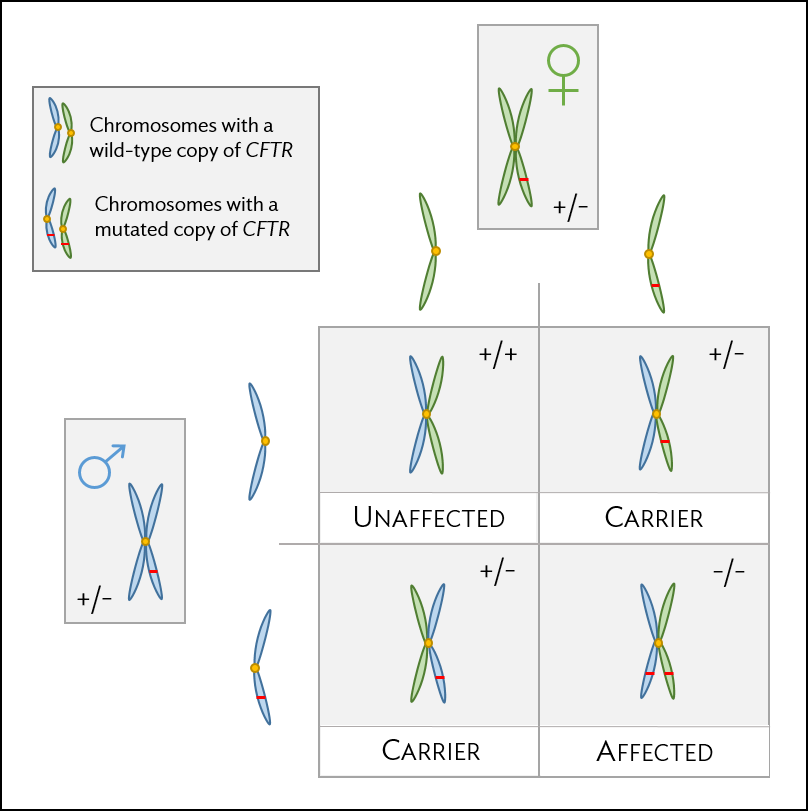
\includegraphics[width= 0.75\textwidth]{ch_probability_oi_biostat/figures/cfInheritance/cfInheritance.png}
	\caption{Pattern of CF inheritance for a child of two unaffected carriers}
	\label{fig:cfInheritance}
\end{figure}

\begin{exercise}
Suppose the father has CF and the mother is an unaffected carrier. What is the probability that their child will be affected by the disease?

\textit{Solution:}  Since the father has CF, he must have two affected copies; he will always pass along a defective copy of the gene.  Since the mother will pass along a defective copy half of the time, the child will be affected half of the time, or with probability $1/2$.

\end{exercise}

\subsection{Probability}

% \index{random phenomena |(}

Probability is used to assign a level of uncertainty to the outcomes of phenomena that either happen randomly (e.g. rolling dice, inheriting of disease alleles), or appear random because of a lack of understanding about exactly how the phenomenon occurs (e.g. an obese teenager with high blood pressure developing cardiovascular disease later in life). Modeling these complex phenomena as random can be useful, and in either case, the interpretation of probability is the same: the chance that some event will happen in the future.

Mathematicians and philosophers have struggled for centuries to arrive at a clear statement of how probability is defined, or what it means.  In this text we use the most common definition, which also has the clearest interpretation.

\begin{termBox}{\tBoxTitle{Probability}
The \term{probability} of an outcome is the proportion of times the outcome would occur if the random phenomenon could be observed an infinite number of times.}
\end{termBox}

\index{Law of Large Numbers |(}

\begin{figure}[bt]
	\centering
	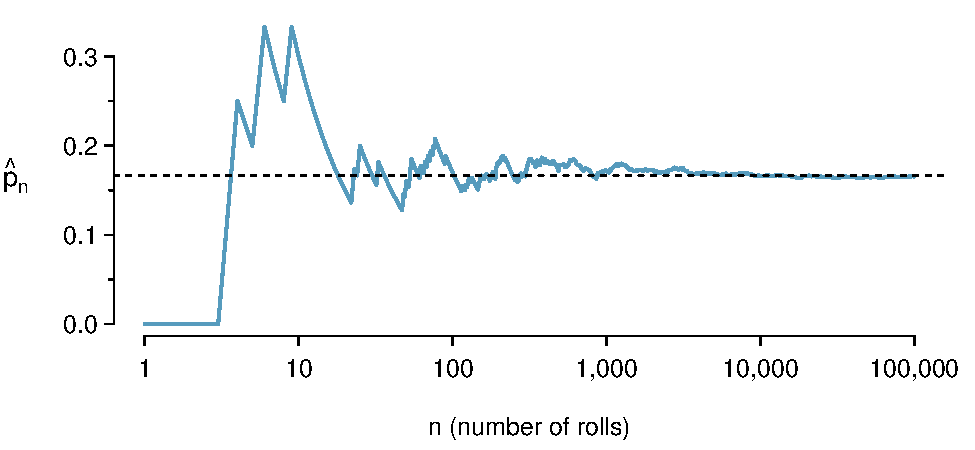
\includegraphics[width=0.85\textwidth]{ch_probability_oi_biostat/figures/dieProp/dieProp}
	\caption{The fraction of die rolls that are \resp{1} at each stage in a simulation. The proportion tends to get closer to the probability $1/6 \approx 0.167$ as the number of rolls increases.}
	\label{fig:dieProp}
\end{figure}

This definition of probability can be illustrated by rolling a die many times. Let $\hat{p}_n$ be the proportion of outcomes that are \resp{1} after the first $n$ rolls. As the number of rolls increases, $\hat{p}_n$ will converge to the probability of rolling a \resp{1}, $p = 1/6$. Figure~\ref{fig:dieProp} shows this convergence for 100,000 die rolls. The tendency of $\hat{p}_n$ to stabilize around $p$ is described by the \term{Law of Large Numbers}. The behavior shown in Figure~\ref{fig:dieProp} matches most people's intuition about probability, but proving mathematically that the behavior is always true is surprisingly difficult and beyond the level of this text.

Occasionally the proportion will veer off from the probability and appear to defy the Law of Large Numbers, as $\hat{p}_n$ does many times in Figure~\ref{fig:dieProp}. However, these deviations become smaller as the number of rolls increases.

\begin{termBox}{\tBoxTitle{Law of Large Numbers}
As more observations are collected, the proportion $\hat{p}_n$ of occurrences with a particular outcome converges to the probability $p$ of that outcome.}
\end{termBox}

\index{Law of Large Numbers |)}

While it is easy to imagine repeatedly rolling a die to observe the law of large numbers, the interpretation of probability is more hypothetical for examples like disease inheritance, since family sizes are typically small -- if two unaffected carriers were to have many children, then approximately 25\% of their offspring would suffer from CF.

Probability is defined as a proportion, and it always takes values between 0~and~1 (inclusively). It may also be displayed as a percentage between 0\% and 100\%. The notation $p$ is the probability of rolling a \resp{1}. We can also write this probability as
\begin{eqnarray*}
P(\text{rolling a \resp{1}})
\end{eqnarray*}
\marginpar[\raggedright\vspace{-13mm}

$P(A)$\vspace{1mm}\\\footnotesize Probability of\\outcome $A$]{\raggedright\vspace{-13mm}

$P(A)$\vspace{1mm}\\\footnotesize Probability of\\outcome $A$}As we become more comfortable with this notation, we will abbreviate it further. For instance, if it is clear that the process is ``rolling a die'', we could abbreviate $P($rolling a \resp{1}$)$ as~$P($\resp{1}$)$.  We also have a notation for an event itself, so the event $A$ of rolling a 1 will be written as $A = \{\text{rolling a \resp{1}}\}$, with associated probability $P(A)$. 

\index{random phenomena|)}

\subsection{Disjoint or mutually exclusive outcomes}

\index{disjoint|(}
\index{mutually exclusive|(}

Two outcomes are called \term{disjoint} or \term{mutually exclusive} if they cannot both happen at the same time. When rolling a die, the outcomes \resp{1} and \resp{2} are disjoint since they cannot both occur.  However, the outcomes \resp{1} and ``rolling an odd number'' are not disjoint since both occur if the outcome of the roll is a \resp{1}. Similarly, for the CF example, the outcomes of a child being affected and having a mutated copy of \textit{CFTR} are not disjoint. The terms \emph{disjoint} and \emph{mutually exclusive} are equivalent and interchangeable. 

When rolling a die, the outcomes \resp{1} and \resp{2} are disjoint. We compute the probability that one of these outcomes will occur by adding their separate probabilities:
\begin{eqnarray*}
P(\text{\resp{1} or \resp{2}}) = P(\text{\resp{1}})+P(\text{\resp{2}}) = 1/6 + 1/6 = 1/3
\end{eqnarray*}
What about  the probability of rolling a \resp{1}, \resp{2}, \resp{3}, \resp{4}, \resp{5}, or \resp{6}? Here again, all of the outcomes are disjoint so we add the probabilities:
\begin{eqnarray*}
&&P(\text{\resp{1} or \resp{2} or \resp{3} or \resp{4} or \resp{5} or \resp{6}}) \\
	&&\quad= P(\text{\resp{1}})+P(\text{\resp{2}})+P(\text{\resp{3}})+P(\text{\resp{4}})+P(\text{\resp{5}})+P(\text{\resp{6}}) \\
	&&\quad= 1/6 + 1/6 + 1/6 + 1/6 + 1/6 + 1/6 = 1.
\end{eqnarray*}

For the CF example, there are two mutually exclusive outcomes for which a child of two carriers can also be a carrier -- a child can either receive an affected copy of \textit{CFTR} from the mother and a normal copy from the father, or vice versa (since each parent can only contribute one allele). Thus, the probability that a child will be an unaffected carrier is $(1/2) + (1/2) = 1/4$.

The \term{Addition Rule} guarantees the accuracy of this approach when the outcomes are disjoint. 

\begin{termBox}{\tBoxTitle{Addition Rule of disjoint outcomes} If $A_1$ and $A_2$ represent two disjoint outcomes, then the probability that either one of them occurs is given by
\begin{eqnarray*}
P(A_1\text{ or } A_2) = P(A_1) + P(A_2)
\end{eqnarray*}
If there are $k$ disjoint outcomes $A_1$, ..., $A_k$, then the probability that one of these outcomes will occur is
\begin{eqnarray}
P(A_1) + P(A_2) + \cdots + P(A_k)
\end{eqnarray}
}
\end{termBox}

\index{event|(}


Probability problems rarely consider individual outcomes and instead often deal with \indexthis{\emph{sets}}{sets} or \indexthis{\emph{collections}}{collections} of outcomes. Let $A$ represent the event in which a die roll results in \resp{1} or \resp{2} and $B$~represent the event that the die roll is a \resp{4} or a \resp{6}. We write $A$ as the set of outcomes $\{$\resp{1},~\resp{2}$\}$ and $B=\{$\resp{4}, \resp{6}$\}$. These sets are commonly called \termsub{events}{event}. Because $A$ and $B$ have no elements in common, they are disjoint events. $A$ and $B$ are represented in Figure~\ref{fig:disjointEvents}.

\begin{figure}[hhh]
\centering
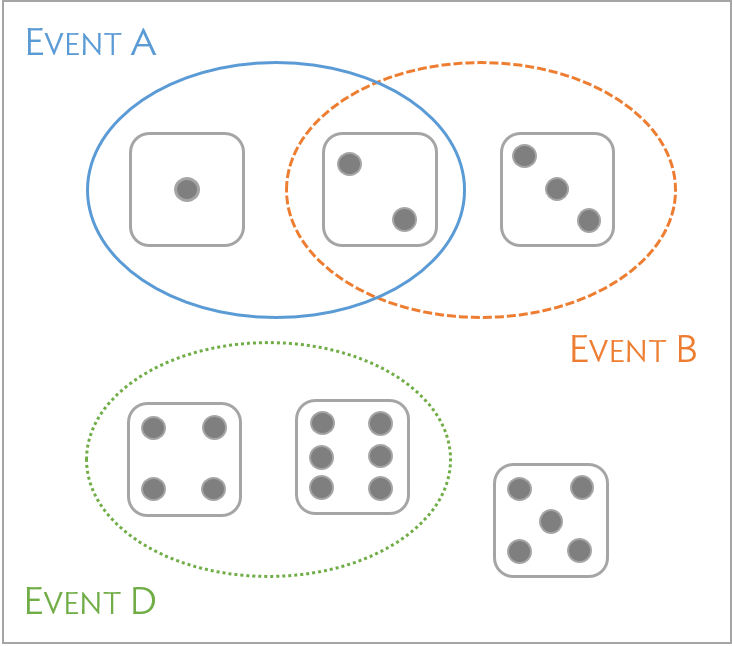
\includegraphics[width=0.55\textwidth]{ch_probability_oi_biostat/figures/disjointEvents/disjointEvents.png}
\caption{Three events, $A$, $B$, and $D$, consist of outcomes from rolling a die. $A$ and $B$ are disjoint since they do not have any outcomes in common.}
\label{fig:disjointEvents}
\end{figure}

The Addition Rule applies to both disjoint outcomes and disjoint events. The probability that one of the disjoint events $A$ or $B$ occurs is the sum of the separate probabilities:
\begin{align*}
P(A\text{ or }B) = P(A) + P(B) = 1/3 + 1/3 = 2/3
\end{align*}

\begin{exercise}
(a) Verify the probability of event $A$, $P(A)$, is $1/3$ using the Addition Rule. (b) Do the same for event $B$.\footnote{(a) $P(A) = P($\resp{1} or \resp{2}$) = P($\resp{1}$) + P($\resp{2}$) = \frac{1}{6} + \frac{1}{6} = \frac{2}{6} = \frac{1}{3}$. (b) Similarly, $P(B) = 1/3$.}
\end{exercise}

\begin{exercise} \label{exerExaminingDisjointSetsABD}
(a) Using Figure~\ref{fig:disjointEvents} as a reference, which outcomes are represented by event $D$? (b) Are events $B$ and $D$ disjoint? (c) Are events $A$ and $D$ disjoint?\footnote{(a)~Outcomes \resp{2} and \resp{3}. (b)~Yes, events $B$ and $D$ are disjoint because they share no outcomes. (c)~The events $A$ and $D$ share an outcome in common, \resp{2}, and so are not disjoint.}
\end{exercise}

\begin{exercise}
In Guided Practice~\ref{exerExaminingDisjointSetsABD}, you confirmed $B$ and $D$ from Figure~\ref{fig:disjointEvents} are disjoint. Compute the probability that event $B$ or event $D$~occurs.\footnote{Since $B$ and $D$ are disjoint events, use the Addition Rule: $P(B$ or $D) = P(B) + P(D) = \frac{1}{3} + \frac{1}{3} = \frac{2}{3}$.}
\end{exercise}

%DH: \textit{DH: Should we add more genetics problems here?  I have removed the email example because of the possible confusion between events involving sampling from a population vs a study sample.  If we think we can make that clear, we can use examples from famuss, perhaps by posing a problem of sampling members from the study participants.  Note also that this is moving more slowly than the Stat 102 notes, but we did show some of this material on the blackboard. If we use this chapter in 102, perhaps we can move quickly to more complicated examples.}

%JV: \textit{JV: Perhaps famuss examples could be added later in a more complicated context, to keep the chapter from moving too slowly at this point.}

\index{event|)}
\index{disjoint|)}
\index{mutually exclusive|)}

\subsection{Probabilities when events are not disjoint}

\term{Venn diagrams} are useful when outcomes can be categorized as ``in'' or ``out'' for two or three variables, attributes, or random processes. The Venn diagram in Figure~\ref{fig:cardsDiamondFaceVenn} uses one oval to represent diamonds and another to represent face cards (the cards labeled jacks, queens, and kings); if a card is both a diamond and a face card, it falls into the intersection of the ovals.

\begin{table}[h]
\centering
\begin{tabular}{lll lll lll lll l}
\resp{2$\clubsuit$} & \resp{3$\clubsuit$} & \resp{4$\clubsuit$} & \resp{5$\clubsuit$} & \resp{6$\clubsuit$} & \resp{7$\clubsuit$} & \resp{8$\clubsuit$} & \resp{9$\clubsuit$} & \resp{10$\clubsuit$} & \resp{J$\clubsuit$} & \resp{Q$\clubsuit$} & \resp{K$\clubsuit$} & \resp{A$\clubsuit$}  \\
\color{redcards} \resp{2$\diamondsuit$} & \color{redcards}\resp{3$\diamondsuit$} & \color{redcards}\resp{4$\diamondsuit$} & \color{redcards}\resp{5$\diamondsuit$} & \color{redcards}\resp{6$\diamondsuit$} & \color{redcards}\resp{7$\diamondsuit$} & \color{redcards}\resp{8$\diamondsuit$} & \color{redcards}\resp{9$\diamondsuit$} & \color{redcards}\resp{10$\diamondsuit$} & \color{redcards}\resp{J$\diamondsuit$} & \color{redcards}\resp{Q$\diamondsuit$} & \color{redcards}\resp{K$\diamondsuit$} & \color{redcards}\resp{A$\diamondsuit$} \\
\color{redcards}\resp{2$\heartsuit$} & \color{redcards}\resp{3$\heartsuit$} & \color{redcards}\resp{4$\heartsuit$} & \color{redcards}\resp{5$\heartsuit$} & \color{redcards}\resp{6$\heartsuit$} & \color{redcards}\resp{7$\heartsuit$} & \color{redcards}\resp{8$\heartsuit$} & \color{redcards}\resp{9$\heartsuit$} & \color{redcards}\resp{10$\heartsuit$} & \color{redcards}\resp{J$\heartsuit$} & \color{redcards}\resp{Q$\heartsuit$} & \color{redcards}\resp{K$\heartsuit$} & \color{redcards}\resp{A$\heartsuit$} \\
\resp{2$\spadesuit$} & \resp{3$\spadesuit$} & \resp{4$\spadesuit$} & \resp{5$\spadesuit$} & \resp{6$\spadesuit$} & \resp{7$\spadesuit$} & \resp{8$\spadesuit$} & \resp{9$\spadesuit$} & \resp{10$\spadesuit$} & \resp{J$\spadesuit$} & \resp{Q$\spadesuit$} & \resp{K$\spadesuit$} & \resp{A$\spadesuit$}
\end{tabular}
\caption{A \indexthis{regular deck of 52 cards}{deck of cards} is split into four \term{suits}: $\clubsuit$ (club), {\color{redcards}$\diamondsuit$} (diamond), {\color{redcards}$\heartsuit$} (heart), $\spadesuit$ (spade). Each suit has its 13 cards labeled: \resp{2}, \resp{3}, ..., \resp{10}, \resp{J} (jack), \resp{Q} (queen), \resp{K} (king), and \resp{A} (ace). Thus, each card is a unique combination of a suit and a label, e.g. {\color{redcards}\resp{4$\heartsuit$}} and \resp{J$\clubsuit$}. %The cards that are {\color{redcards}$\diamondsuit$} or {\color{redcards}$\heartsuit$} are typically colored {\color{redcards}red} while the other two suits are typically colored black.
	}
\label{deckOfCards}
\end{table}

\begin{figure}[h]
	\centering
	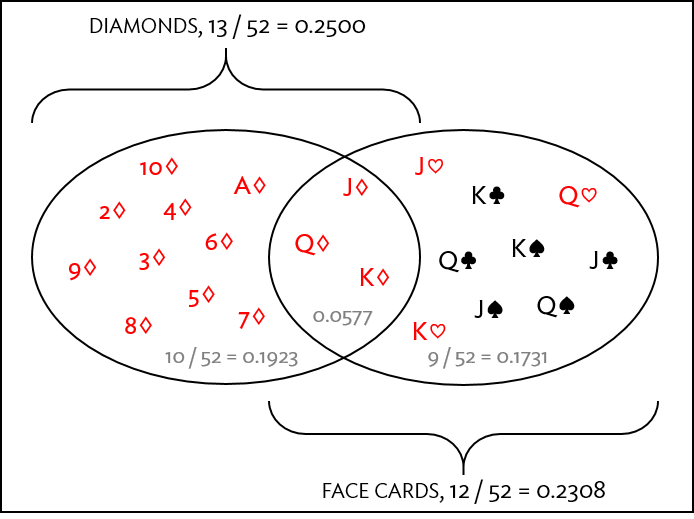
\includegraphics[width=0.65\textwidth]{ch_probability_oi_biostat/figures/cardsDiamondFaceVenn/cardsDiamondFaceVenn.png}
	\caption{A Venn diagram for diamonds and face cards.}
	\label{fig:cardsDiamondFaceVenn}
\end{figure}

%\begin{exercise}
%Using Figure~\ref{cardsDiamondFaceVenn}, verify $P($face card$) = 12/52=3/13$.\footnote{The Venn diagram shows face cards split up into ``face card but not {\color{redcards}$\diamondsuit$}'' and ``face card and {\color{redcards}$\diamondsuit$}''. Since these correspond to disjoint events, $P($face card$)$ is found by adding the two corresponding probabilities: $\frac{3}{52} + \frac{9}{52} = \frac{12}{52} = \frac{3}{13}$.}
%\end{exercise}

\begin{exercise}
	(a) What is the probability that a randomly selected card is a diamond? (b)~What is the probability that a randomly selected card is a face card?\footnote{(a) There are 52 cards and 13 diamonds. If the cards are thoroughly shuffled, each card has an equal chance of being drawn, so the probability that a randomly selected card is a diamond is $P({\color{redcards}\diamondsuit}) = \frac{13}{52} = 0.250$. (b)~Likewise, there are 12 face cards, so $P($face card$) = \frac{12}{52} = \frac{3}{13} = 0.231$.}
\end{exercise}

Let $A$ represent the event that a randomly selected card is a diamond and $B$ represent the event that it is a face card. Events $A$ and $B$ are not disjoint -- the cards {\color{redcards}$J\diamondsuit$}, {\color{redcards}$Q\diamondsuit$}, and {\color{redcards}$K\diamondsuit$} fall into both categories. 

As a result, adding the probabilities of the two events together is not sufficient to calculate $P(A \ \text{or} \ B)$:

\begin{eqnarray*}
	P(A) + P(B) = P({\color{redcards}\diamondsuit}) + P(\text{face card}) = 12/52 + 13/52
	\label{overCountFaceDiamond}
\end{eqnarray*}

Instead, a small modification is necessary. The three cards that are in both events were counted twice, once in each probability. To correct the double counting, subtract the probability that both events occur:

\begin{eqnarray}
P(A\text{ or } B) &=&P(\text{face card or }{\color{redcards}\diamondsuit})  \notag \\
 &=& P(\text{face card}) + P({\color{redcards}\diamondsuit}) - P(\text{face card and }{\color{redcards}\diamondsuit}) \label{diamondFace} \\
 &=& 13/52 + 12/52 - 3/52 \notag \\
 &=& 22/52 = 11/26 \notag
\end{eqnarray}
Equation~(\ref{diamondFace}) is an example of the \term{General Addition Rule}. 

\begin{termBox}{\tBoxTitle{General Addition Rule} If $A$ and $B$ are any two events, disjoint or not, then the probability that at least one of them will occur is
\begin{eqnarray}
P(A\text{ or }B) = P(A) + P(B) - P(A\text{ and }B)
\label{generalAdditionRule}
\end{eqnarray}
where $P(A$ and $B)$ is the probability that both events occur.}
\end{termBox}


\begin{tipBox}{\tipBoxTitle{``or'' is inclusive}
Note that in the language of statistics, "or" is in inclusive such that $A$ or $B$ occurs means $A$, $B$, or both $A$ and $B$ occur.}
\end{tipBox}

\begin{exercise}
(a) If $A$ and $B$ are disjoint, describe why this implies $P(A$ and $B) = 0$. (b) Using part (a), verify that the General Addition Rule simplifies to the simpler Addition Rule for disjoint events if $A$ and $B$ are disjoint.\footnote{(a) If $A$ and $B$ are disjoint, $A$ and $B$ can never occur simultaneously. (b) If $A$ and $B$ are disjoint, then the last term of Equation~(\ref{generalAdditionRule}) is 0 (see part (a)) and we are left with the Addition Rule for disjoint events.}
\end{exercise}

\begin{exercise}
{Human immunodeficiency virus (HIV) and tuberculosis (TB) affect substantial proportions of the population in certain areas of the developing world. Individuals sometimes have both diseases (are co-infected); children of HIV-infected mothers may have HIV (be HIV$^+$) and TB can spread from one family member to another.  In a mother child pair, let $A = \{\text{ the mother has HIV } \}$,  $B = \{\textrm{ the mother has TB } \}$, $C = \{\text{ the child has HIV } \}$,  $D = \{\text{ the child has TB } \}$.  Write out the definitions of the events $A \text{ or } B$, $A \text{ and } B$, $A \text{ and } C$, $A \text{ or } D$.}\footnote{Events $A$ or $B$: the mother has HIV, the mother has TB, or the mother has both HIV and TB. Events $A$ and $B$: the mother has both HIV and TB. Events $A$ and $C$: The mother has HIV and the child has HIV. $A$ or $D$: The mother has HIV, the child has TB, or the mother has HIV and the child has TB.}

\end{exercise}

\subsection{Probability distributions}

A \term{probability distribution} is a table of all disjoint outcomes and their associated probabilities. Table~\ref{diceProb} shows the probability distribution for the sum of two dice. 

\begin{table}[h] \small
\centering
\begin{tabular}{l ccc ccc ccc cc}
  \hline
  \ \vspace{-3mm} \\
Dice sum\vspace{0.3mm} & 2 & 3 & 4 & 5 & 6 & 7 & 8 & 9 & 10 & 11 & 12  \\
Probability & $\frac{1}{36}$ & $\frac{2}{36}$ & $\frac{3}{36}$ & $\frac{4}{36}$ & $\frac{5}{36}$ & $\frac{6}{36}$ & $\frac{5}{36}$ & $\frac{4}{36}$ & $\frac{3}{36}$ & $\frac{2}{36}$ & $\frac{1}{36}$\vspace{1mm} \\
   \hline
\end{tabular}
\caption{Probability distribution for the sum of two dice.}
\label{diceProb}
\end{table}

\begin{termBox}{\tBoxTitle{Rules for probability distributions}
A probability distribution is a list of the possible outcomes with corresponding probabilities that satisfies three rules: \vspace{-2mm}
\begin{enumerate}
\setlength{\itemsep}{0mm}
\item The outcomes listed must be disjoint.
\item Each probability must be between 0 and 1.
\item The probabilities must total to 1. \vspace{1mm}
\end{enumerate}}
\end{termBox}

Chapter~\ref{introductionToData} emphasized the importance of plotting data to provide quick summaries. Probability distributions can also be summarized in a bar plot. The probability distribution for the sum of two dice is shown in Table~\ref{diceProb} and plotted in Figure~\ref{diceSumDist}.

\begin{figure}
\centering
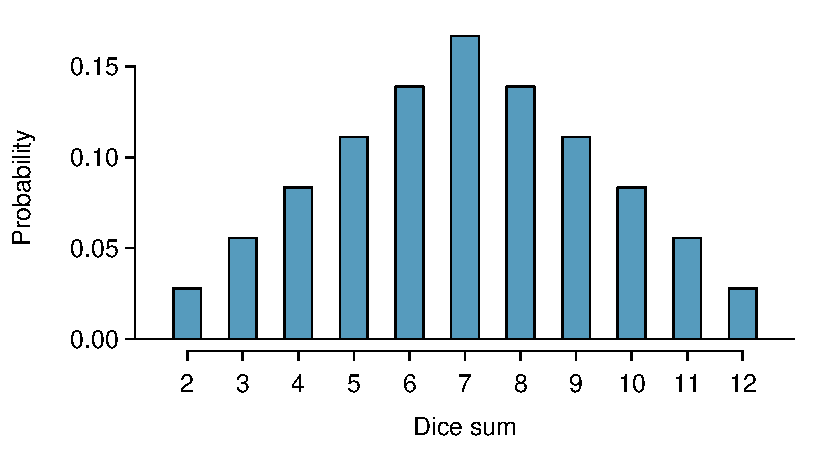
\includegraphics[width=0.73\textwidth]{ch_probability_oi_biostat/figures/diceSumDist/diceSumDist}
\caption{The probability distribution of the sum of two dice.}
\label{diceSumDist}
\end{figure}

In this bar plot, the bar heights represent the probabilities of outcomes. If the outcomes are numerical and discrete, it can be visually convenient to make a bar plot that resembles a histogram, such as in the case of the sum of two dice.  

A graph of probability distribution can quickly convey important information about a distribution quickly. For example, the distribution of birth weights for 3,999,386 live births in the United States in 2010 is shown in Figure \ref{fig:birthwtMarginalDist}.  The data are available as part of the US CDC National Vital Statistics System.\footnote{\url{http://205.207.175.93/vitalstats/ReportFolders/reportFolders.aspx}} The graph of the distribution shows that while most babies born weighed between 2000 and 5000 grams (2 to 5 kg), there were both small (less than 1000 grams) and large (greater than 5000 grams) babies. Pediatricians consider birth weights between 2.5 and 5 kg as normal. 

%JV: \textit{JV: Citation for normal birthwt?}

\begin{figure}[h]
	\includegraphics[width=\textwidth]{ch_probability_oi_biostat/figures/birthwtMarginalDist/birthwtMarginalDist.pdf}
	\caption{Distribution of birth weights (in grams) of babies born in the US in 2010}
	\label{fig:birthwtMarginalDist}
\end{figure}

%JV: \textit{JV: Text in the birthweight plot is very small, in order to accommodate the number of bars... If you agree that bars can be reduced, adjust the marginal dist table and I can re-size the plot.}

\subsection{Complement of an event}

Rolling a die produces a value in the set $\{$\resp{1}, \resp{2}, \resp{3}, \resp{4}, \resp{5}, \resp{6}$\}$. This set of all possible outcomes is called the \term{sample space} ($S$)\marginpar[\raggedright\vspace{-5mm}

$S$\\\footnotesize Sample space]{\raggedright\vspace{-5mm}

$S$\\\footnotesize Sample space}\index{S@$S$} for rolling a die. 

Let $D=\{$\resp{2}, \resp{3}$\}$ represent the event that the outcome of a die roll is \resp{2} or \resp{3}. The \term{complement}\marginpar[\raggedright\vspace{0.2mm}

$A^c$\\\footnotesize Complement\\of outcome $A$]{\raggedright\vspace{0.2mm}

$A^c$\\\footnotesize Complement\\of outcome $A$}\index{Ac@$A^c$} of $D$ represents all outcomes in our sample space that are not in $D$, which is denoted by $D^c = \{$\resp{1}, \resp{4}, \resp{5}, \resp{6}$\}$. That is, $D^c$ is the set of all possible outcomes not already included in $D$. Figure~\ref{fig:complementOfD} shows the relationship between $D$, $D^c$, and the sample space $S$. 

\begin{figure}[hht]
\centering
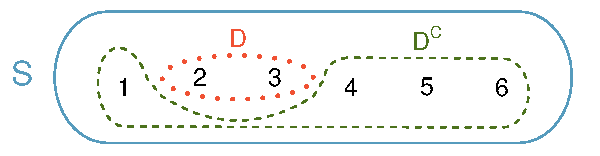
\includegraphics[width=0.55\textwidth]{ch_probability_oi_biostat/figures/complementOfD/complementOfD}
\caption{Event $D=\{$\resp{2}, \resp{3}$\}$ and its complement, $D^c = \{$\resp{1}, \resp{4}, \resp{5}, \resp{6}$\}$. $S$~represents the sample space, which is the set of all possible events.}
\label{fig:complementOfD}
\end{figure}

\begin{exercise}
(a) Compute $P(D^c) = P($rolling a \resp{1}, \resp{4}, \resp{5}, or \resp{6}$)$. (b) What is $P(D) + P(D^c)$?\footnote{(a)~The outcomes are disjoint and each has probability $1/6$, so the total probability is $4/6=2/3$. (b)~We can also see that $P(D)=\frac{1}{6} + \frac{1}{6} = 1/3$. Since $D$ and $D^c$ are disjoint, $P(D) + P(D^c) = 1$.}
\end{exercise}

\begin{exercise}
Events $A=\{$\resp{1}, \resp{2}$\}$ and $B=\{$\resp{4}, \resp{6}$\}$ are shown in Figure~\ref{fig:disjointEvents} on page~\pageref{fig:disjointEvents}. (a) Write out what $A^c$ and $B^c$ represent. (b)~Compute $P(A^c)$ and $P(B^c)$. (c)~Compute $P(A)+P(A^c)$ and $P(B)+P(B^c)$.\footnote{Brief solutions: (a)~$A^c=\{$\resp{3}, \resp{4}, \resp{5}, \resp{6}$\}$ and $B^c=\{$\resp{1}, \resp{2}, \resp{3}, \resp{5}$\}$. (b)~Noting that each outcome is disjoint, add the individual outcome probabilities to get $P(A^c)=2/3$ and $P(B^c)=2/3$. (c)~$A$~and~$A^c$ are disjoint, and the same is true of $B$~and~$B^c$. Therefore, $P(A) + P(A^c) = 1$ and $P(B) + P(B^c) = 1$.}
\end{exercise}

A complement of an event $A$ is constructed to have two very important properties: (i) every possible outcome not in $A$ is in $A^c$, and (ii) $A$ and $A^c$ are disjoint. Property (i) implies
\begin{eqnarray}
P(A\text{ or }A^c) = 1
\label{complementSumTo1}
\end{eqnarray}
That is, if the outcome is not in $A$, it must be represented in $A^c$. We use the Addition Rule for disjoint events to apply Property (ii):
\begin{eqnarray}
P(A\text{ or }A^c) = P(A) + P(A^c)
\label{complementDisjointEquation}
\end{eqnarray}
Combining Equations~(\ref{complementSumTo1}) and~(\ref{complementDisjointEquation}) yields a useful relationship between the probability of an event and its complement.

\begin{termBox}{\tBoxTitle{Complement}
The complement of event $A$ is denoted $A^c$, and $A^c$ represents all outcomes not in~$A$. $A$ and $A^c$ are mathematically related: \vspace{-2mm}
\begin{eqnarray}\label{complement}
P(A) + P(A^c) = 1, \quad\text{i.e.}\quad P(A) = 1-P(A^c)
\end{eqnarray}\vspace{-6.5mm}}
\end{termBox}

In simple examples, computing either $A$ or $A^c$ is feasible in a few steps. However, as problems grow in complexity, using the relationship between an event and its complement can be a useful strategy.

\begin{exercise}
Let $A$ represent the event in which two dice are rolled and their total is less than \resp{12}. (a) What does the event $A^c$ represent? (b) Determine $P(A^c)$ from Table~\ref{diceProb} on page~\pageref{diceProb}. (c) Determine $P(A)$.\footnote{(a)~The complement of $A$: when the total is equal to \resp{12}. (b)~$P(A^c) = 1/36$. (c)~Use the probability of the complement from part (b), $P(A^c) = 1/36$, and Equation~(\ref{complement}): $P($less than \resp{12}$) = 1 - P($\resp{12}$) = 1 - 1/36 = 35/36$.}
\end{exercise}

\begin{exercise} Consider again the probabilities from Table~\ref{diceProb} and rolling two dice. Find the following probabilities: (a)~The sum of the dice is \emph{not} \resp{6}. (b)~The sum is at least \resp{4}. That is, determine the probability of the event $B=\{$\resp{4}, \resp{5}, ..., \resp{12}$\}$. (c) The sum is no more than \resp{10}. That is, determine the probability of the event $D=\{$\resp{2}, \resp{3}, ..., \resp{10}$\}$.\footnote{(a)~First find $P($\resp{6}$)=5/36$, then use the complement: $P($not \resp{6}$) = 1 - P($\resp{6}$) = 31/36$.

(b)~First find  the complement, which requires much less effort: $P($\resp{2} or \resp{3}$)=1/36+2/36=1/12$. Then calculate $P(B) = 1-P(B^c) = 1-1/12 = 11/12$.

(c)~As before, finding the complement is the more direct way to determine $P(D)$. First find $P(D^c) = P($\resp{11} or \resp{12}$)=2/36 + 1/36=1/12$. Then calculate $P(D) = 1 - P(D^c) = 11/12$.}
\end{exercise}

\begin{comment}

\textit{JV: I agree that this example requires too much explanation for what should be a relatively short point... Will leave as-is for now.}

Sometimes, information from a graph can be combined with using the complement of an event to calculate approximate probabilities. The gestational age of a newborn is the time between conception and birth. Because of the obvious difficulty of determining the exact date of conception, gestational ages are typically recorded in weeks. Figure \ref{fig:gestageMarginalDist} is the graphical representation of the distribution of gestational ages for the  3,999,386 babies born in 2010.  Babies born between 38 and 42 weeks of gestational age are considered normal, but the term `full term' is used for births between 39 and 40 weeks gestational age.  The graph shows that approximately 30\% of births occur at 39 weeks, and slightly less than 30\% occur at 40 weeks, so approximately 50\% of babies are considered full term.  Instead of adding up the heights of the bars for gestational ages outside the full term range, using the complement of the event of a full term birth, it is clear that approximately 50\% of births not considered full term.

\begin{figure}
  \centering
  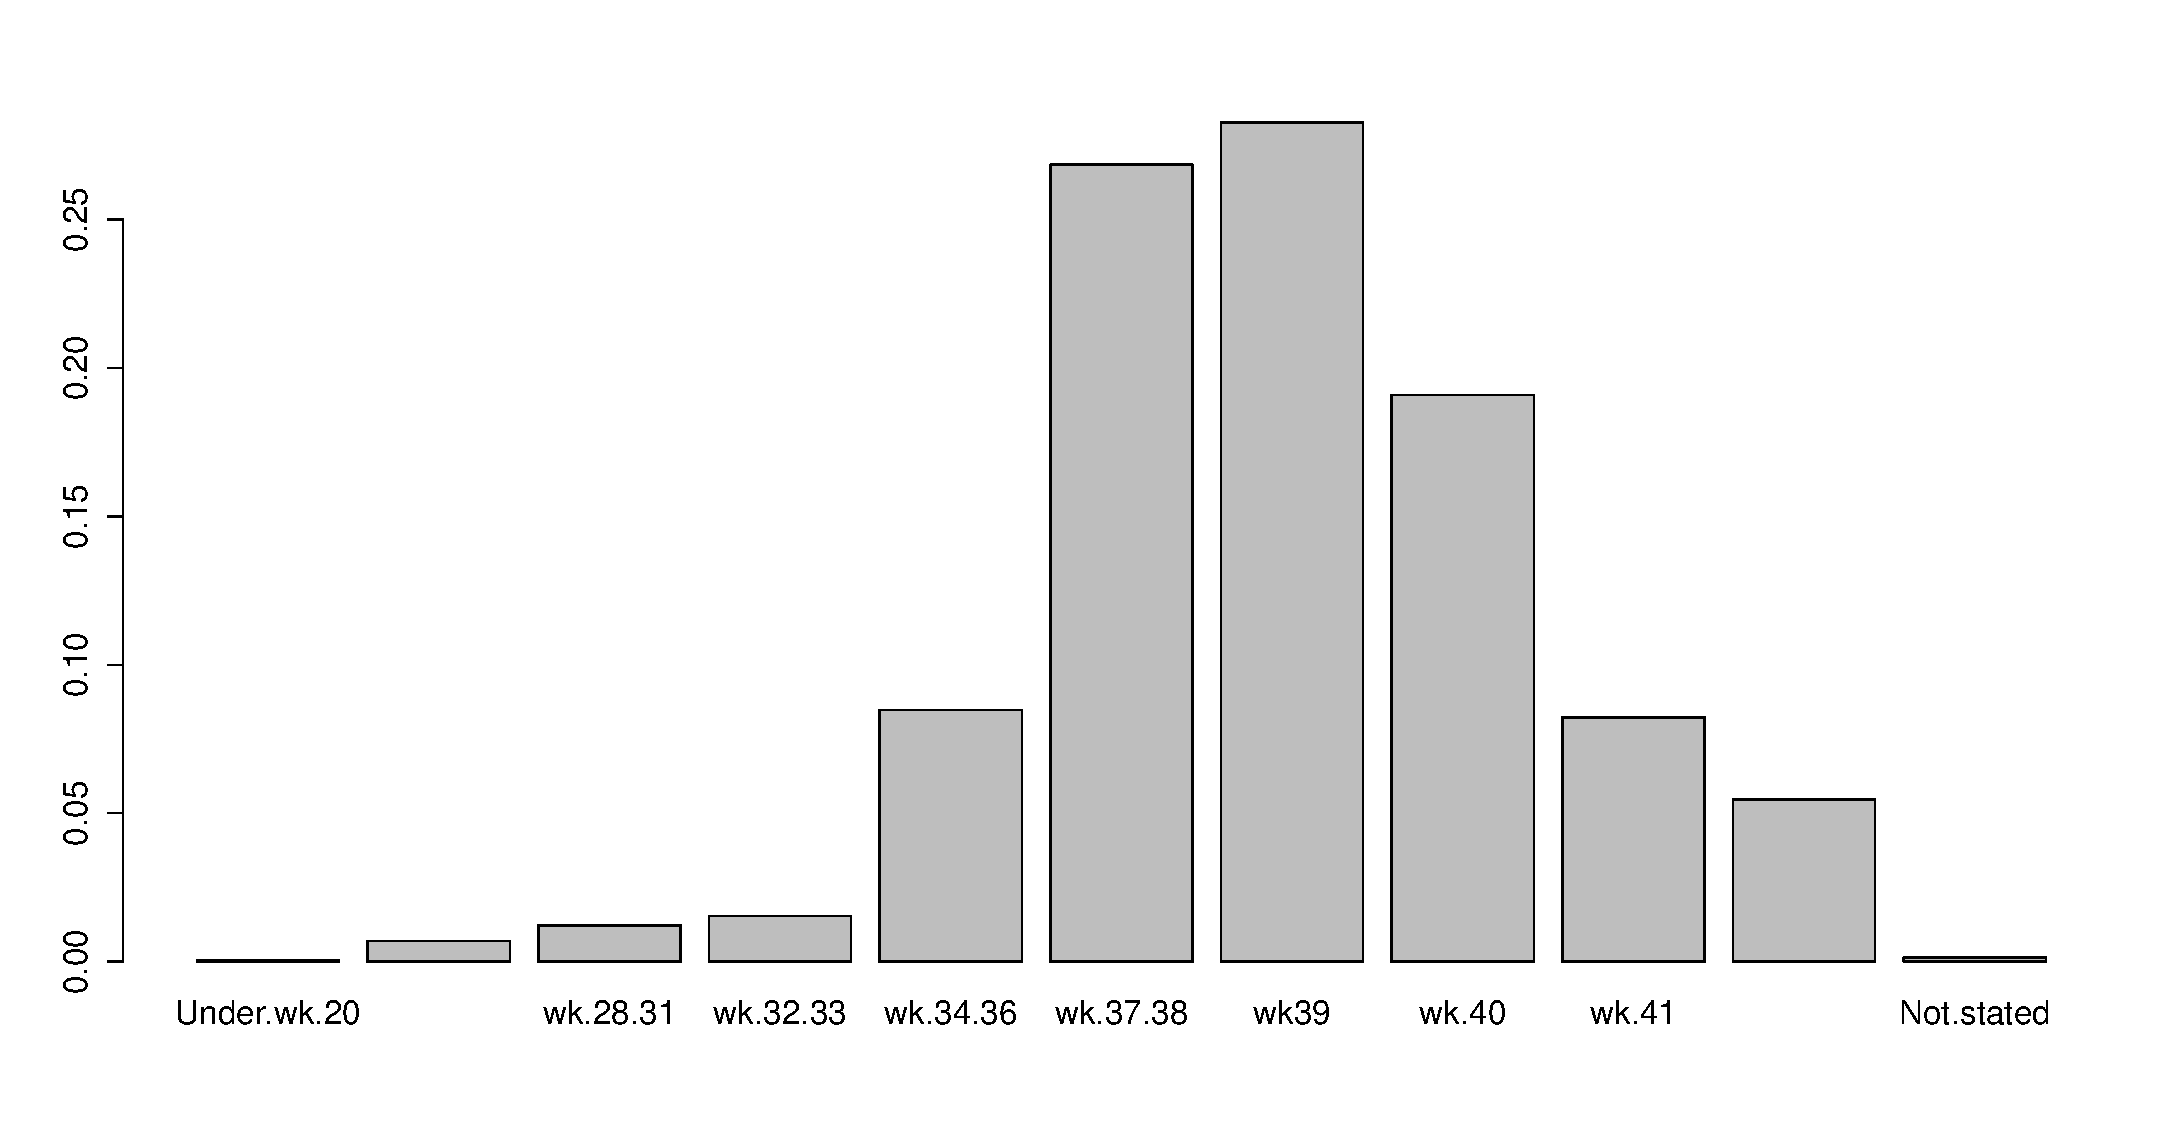
\includegraphics[width=0.75\textwidth]{ch_probability_oi_biostat/figures/gestageMarginalDist/gestageMarginalDist.pdf}
  \caption{Distribution of gestational age for live births in the US in 2010, measured in weeks}
  \label{fig:gestageMarginalDist}
\end{figure}

% R script for creating figure stored with the figure; needs to be improved

The distribution of gestational age is shown in tabular form in Table \ref{gestageMarginalDistTable}.  The table shows the exact value of the proportion of babies born at 39 or 40 weeks (0.47), but when examining the important features of a distribution, approximate values are often sufficient.  In some instances, the graph is all that will be available.  Since small probabilities are difficult to read accurately from the graph of a distribution, they are best read from the table.  Pre-term babies are those born at less than 37 weeks gestational age.  Table \ref{gestageMarginalDistTable} shows that the probability of this event is $0.01 + 0.01 + 0.02 + 0.08 = 0.12$.  Of course, even the table shows approximate values, since the small proportion of very premature babies born at less than 20 weeks is rounded to zero.

\textit{DH: two problems with the example: it is too clumsy for what it accomplishes, and I have  included the not stated category in the calculations of the proportions.  This is negligible, but wrong.}

\begin{table}[ht]
\label{gestageMarginalDistTable}
\centering
\begin{tabular}{rr}
  \hline
 & x \\ 
  \hline
Under.wk.20 & 0.00 \\ 
  wk.20.27 & 0.01 \\ 
  wk.28.31 & 0.01 \\ 
  wk.32.33 & 0.02 \\ 
  wk.34.36 & 0.08 \\ 
  wk.37.38 & 0.27 \\ 
  wk39 & 0.28 \\ 
  wk.40 & 0.19 \\ 
  wk.41 & 0.08 \\ 
  wk.42.and.over & 0.05 \\ 
  Not.stated & 0.00 \\ 
   \hline
\end{tabular}
\end{table}

\textit{DH: value labels should be modified}

\textit{DH: not satisfied with the way this example worked out; it should be improved or changed}

\end{comment}

\subsection{Independence}
\label{probabilityIndependence}

Just as variables and observations can be independent, random phenomena can also be independent. Two processes are \term{independent} if knowing the outcome of one provides no information about the outcome of the other. For instance, flipping a coin and rolling a die are two independent processes -- knowing that the coin lands heads up does not help determine the outcome of a die roll. On the other hand, stock prices usually move up or down together, so they are not independent. 

%JV: \textit{JV: Perhaps these examples could be replaced... Ex. dependence of height and weight? independence of other two traits, maybe height and eye color?}

Independence was used implicitly on page~\pageref{CFInheritanceExample} in the second solution to the probability that two carriers will have an affected child with cystic fibrosis. Genes are typically passed along from the mother and father independently, allowing for the assumption that, on average, half of the offspring who receive a mutated gene copy from the mother will also receive a mutated copy from the father.

Example~\ref{probOf2Ones} provides a basic example of two independent processes: rolling two dice. What is the probability that both will be \resp{1}? Suppose one of the dice is blue and the other green. If the outcome of the blue die is a \resp{1}, it provides no information about the outcome of the green die. This question was first encountered in Example~\ref{probOf2Ones} (page~\pageref{probOf2Ones}), with the solution using the following logic: $1/6^{th}$ of the time the blue die is a \resp{1}, and $1/6^{th}$ of \emph{those} times the green die will also be \resp{1}. This is illustrated in Figure~\ref{fig:indepForRollingTwo1s}. Because the rolls are independent, the probabilities of the corresponding outcomes can be multiplied to obtain the final answer: $(1/6)(1/6)=1/36$. This can be generalized to many independent processes. 

\begin{figure}[hht]
\centering
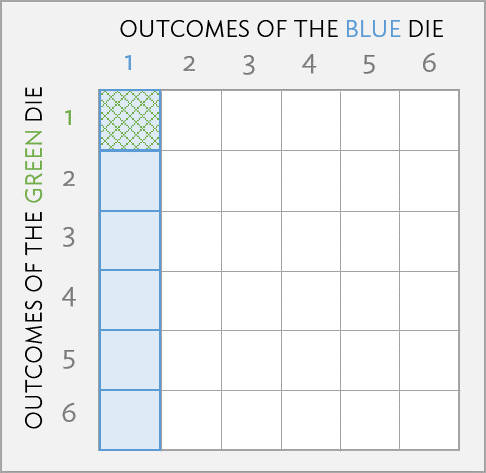
\includegraphics[width=0.5\textwidth]{ch_probability_oi_biostat/figures/indepForRollingTwo1s/indepForRollingTwo1s.png}
\caption{$1/6^{th}$ of the time, the first roll is a \resp{1}. Then $1/6^{th}$ of \emph{those} times, the second roll will also be a \resp{1}.}
\label{fig:indepForRollingTwo1s}
\end{figure}

\begin{exercise}{What if there was also a red die independent of the other two? What is the probability of rolling the three dice and getting all \resp{1}s?}\label{threeDice}
\footnote{The same logic applies from Example~\ref{probOf2Ones}. If $1/36^{th}$ of the time the blue and green dice are both \resp{1}, then $1/6^{th}$ of \emph{those} times the red die will also be \resp{1}, so multiply:
{\begin{align*}
P(blue=\text{\small\resp{1} and } green=\text{\small\resp{1} and } red=\text{\small\resp{1}})
	&= P(blue=\text{\small\resp{1}}) P(green=\text{\small\resp{1}}) P(red=\text{\small\resp{1}}) \\
	&= (1/6) (1/6) (1/6)
	= 1/216
\end{align*}} \vspace{-7mm}
}
\end{exercise}

Guided Practice~\ref{threeDice} illustrates the Multiplication Rule for independent processes. 

\begin{termBox}{\tBoxTitle{\term{Multiplication Rule} for independent processes}
If $A$ and $B$ represent events from two different and independent processes, then the probability that both $A$ and $B$ occur can be calculated as the product of their separate probabilities: \vspace{-1.5mm}
\begin{eqnarray}\label{eqForIndependentEvents}
P(A \text{ and }B) = P(A)  P(B)
\end{eqnarray}
Similarly, if there are $k$ events $A_1$, ..., $A_k$ from $k$ independent processes, then the probability they all occur is\vspace{-1.5mm}
\begin{eqnarray*}
P(A_1) P(A_2) \cdots P(A_k)
\end{eqnarray*}\vspace{-6mm}}
\end{termBox}

In applications to biology or medicine, complicated probability problems are often solved with the simple ideas used in the dice examples. 

%JV: \textit{JV: I think the handedness problems can be put in end-of-chapter exercises. Given this kind of lead-in, we should focus on demonstrating some realistic problems.}

\begin{comment}
\begin{exercise} \label{ex2Handedness}
About 9\% of people are left-handed. Suppose 2 people are selected at random from the U.S. population. Because the sample size of 2 is very small relative to the population, it is reasonable to assume these two people are independent. (a)~What is the probability that both are left-handed? (b)~What is the probability that both are right-handed?\footnote{(a) The probability the first person is left-handed is $0.09$, which is the same for the second person. We apply the Multiplication Rule for independent processes to determine the probability that both will be left-handed: $(0.09) (0.09) = 0.0081$.

(b) It is reasonable to assume the proportion of people who are ambidextrous (both right and left handed) is nearly 0, which results in $P($right-handed$)=1-0.09=0.91$. Using the same reasoning as in part~(a), the probability that both will be right-handed is $(0.91) (0.91) = 0.8281$.}
\end{exercise}

\begin{exercise} \label{ex5Handedness}
Suppose 5 people are selected at random.\footnote{(a)~The abbreviations \resp{RH} and \resp{LH} are used for right-handed and left-handed, respectively. Since each are independent, we apply the Multiplication Rule for independent processes:
\begin{align*}
P(\text{all five are \resp{RH}})
&= P(\text{first = \resp{RH}, second = \resp{RH}, ..., fifth = \resp{RH}}) \\
&= P(\text{first = \resp{RH}})\times P(\text{second = \resp{RH}})\times  \dots \times P(\text{fifth = \resp{RH}}) \\
&= (0.91) (0.91) (0.91) (0.91)(0.91) = 0.624
\end{align*}

(b)~Using the same reasoning as in~(a), $(0.09) (0.09)(0.09)(0.09)(0.09) = 0.0000059$

(c)~Use the complement, $P($all five are \resp{RH}$)$, to answer this question:
\begin{align*}
P(\text{not all \resp{RH}})
	= 1 - P(\text{all \resp{RH}})
	= 1 - 0.624 = 0.376
\end{align*}} \vspace{-1.5mm}
\begin{enumerate}
\setlength{\itemsep}{0mm}
\item[(a)] What is the probability that all are right-handed?
\item[(b)] What is the probability that all are left-handed?
\item[(c)] What is the probability that not all of the people are right-handed?
\end{enumerate}
\end{exercise}

Suppose the variables \var{handedness} and \var{gender} are independent, i.e. knowing someone's \var{gender} provides no useful information about their \var{handedness} and vice-versa. Then we can compute whether a randomly selected person is right-handed and female\footnote{The actual proportion of the U.S. population that is \resp{female} is about 50\%, and so we use 0.5 for the probability of sampling a woman. However, this probability does differ in other countries.} using the Multiplication Rule:
\begin{eqnarray*}
P(\text{right-handed and female}) &=& P(\text{right-handed}) P(\text{female}) \\
&=& (0.91) (0.50) = 0.455
\end{eqnarray*}


\begin{exercise}
Three people are selected at random.\footnote{Brief answers are provided. (a)~This can be written in probability notation as $P($a randomly selected person is male and right-handed$)=0.455$. (b) 0.207. (c) 0.045. (d) 0.0093.} \vspace{-1.5mm}
\begin{enumerate}
\setlength{\itemsep}{0mm}
\item[(a)] What is the probability that the first person is male and right-handed?
\item[(b)] What is the probability that the first two people are male and right-handed?.
\item[(c)] What is the probability that the third person is female and left-handed?
\item[(d)] What is the probability that the first two people are male and right-handed and the third person is female and left-handed?
\end{enumerate}
\end{exercise}

\end{comment}

\begin{example}{\textbf{Mandatory drug testing.} Mandatory drug testing in the workplace is common practice for certain professions, such as air traffic controllers and transportation workers.  A false positive in a drug screening test occurs when the test incorrectly indicates that a screened person is an illegal drug user. Suppose a mandatory drug test has a false-positive rate of 1.2\% (i.e., has probability  0.012 of indicating that an employee is using illegal drugs when that is not the case).  Given 150 employees who are in reality drug free, what is the probability that at least one will (falsely) test positive? Assume that the outcome of one drug test has no affect on the others.}

The solution first defines the event $P(\text{At least 1 "+"})$ in terms of its complement, then uses the multiplication rule to calculate the probability of the complement $P(\text{150 "-"})$.

   \begin{align*} 
   P(\text{At least 1 "+"}) &= P(\text{1 or 2 or 3 \ldots or 150 are "+"}) \\
           &= 1 - P(\text{None are "+"}) \\
           &= 1 - P(\text{150 "-"}) \\
 P(\text{150 are "-"}) &= P(\text{1 is "-"})^{150} \\
           &= (0.988)^{150} = 0.16.
    \end{align*}
   So $P(\text{At least 1 is "+"})  = 1 - P(\text{150 are "-"}) = 0.84.$
 
  %DH: \textit{DH: should we be more formal here in defining events? Also, this is the example that we also solved in R, two different ways.  Those solutions are candidates for the R supplement JV: No, I think it may actually be more intuitive to see events written this way.}

Even when using a test with a small probability of a false positive, the company is more than 80\% likely to incorrectly claim at least one employee is an illegal drug user!

\end{example}

\begin{exercise}
Because of the high likelihood of at least one false positive in company wide drug screening programs, an individual with a positive test is almost always re-tested with a different screening test, one that is more expensive than the first but with a lower false positive probability.  Suppose the second test has a false positive rate of 0.8\%.  What is the probability that an employee who is not using illegal drugs will test positive on both tests?\footnote{The outcomes of the two tests are independent of one another; $P (A\text{ and } B) = P(A) \times P(B)$, where events $A$ and $B$ are the results of the two tests. The probability of a false positive with the first test is 0.012 and 0.008 with the second. Thus, the probability of an employee who is not using illegal drugs testing positive on both tests is $0.012 \times 0.008 = 9.6 \times 10^{-5}$}

\end{exercise}

\begin{figure}[h]
	\centering
	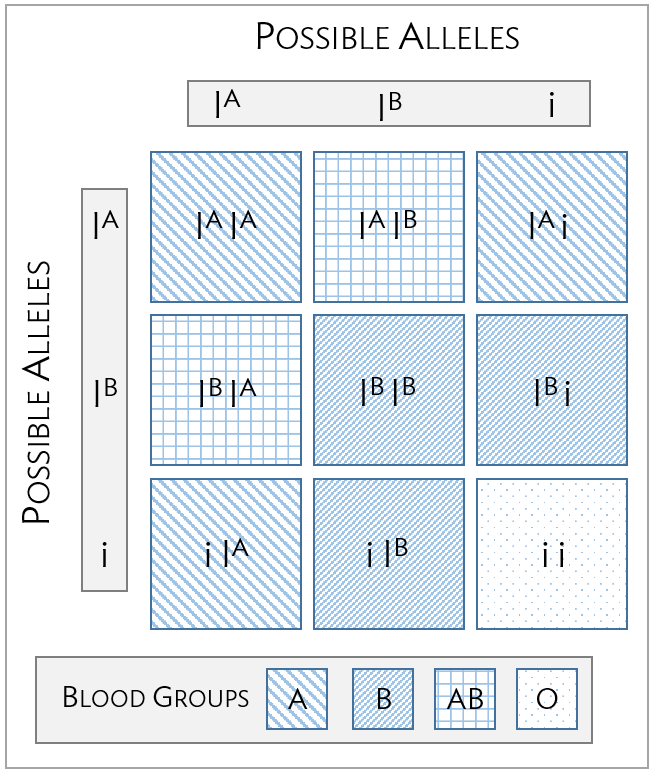
\includegraphics[height= 0.65\textwidth]{ch_probability_oi_biostat/figures/aboInheritance/aboInheritance.png}
	\caption{Inheritance of ABO blood groups.}
	\label{fig:aboInheritance}
\end{figure}

\begin{example}{\textbf{ABO blood groups.} There are four different common blood types (A, B, AB, and O), which are determined by the presence of certain antigens located on cell surfaces. Antigens are substances used by the immune system to recognize self versus non-self; if the immune system encounters antigens not normally found on the body's own cells, it will attack the foreign cells. When patients receive blood transfusions, it is critical that the antigens of transfused cells match those of the patient's, or else an immune system response will be triggered.
		
The ABO blood group system consists of four different blood groups, which describe whether an individual's red blood cells carry the A antigen, B antigen, both, or neither. The ABO gene has three alleles: ${I}^{A}$, ${I}^{B}$, and \textit{i}. The \textit{i} allele is recessive to both ${I}^{A}$ and ${I}^{B}$, and does not produce antigens; thus, an individual with genotype ${I}^{A}i$ is blood group A and an individual with genotype ${I}^{B}i$ is blood group B. The ${I}^{A}$ and ${I}^{B}$ are codominant, such that individuals of ${I}^{A}$${I}^{B}$ genotype are AB. Individuals homozygous for the \textit{i} allele are known as blood group O, with neither A nor B antigens.

Suppose that both members of a couple have Group AB blood.	
\begin{enumerate}[a)]
	\item What is the probability that a child of this couple will have Group A blood?
	\item What is the probability that they have two children with Group A blood?
\end{enumerate}	}

\begin{enumerate}[a)]
	\item An individual with Group AB blood is genotype ${I}^{A}$${I}^{B}$. Two ${I}^{A}$${I}^{B}$ parents can produce children with genotypes ${I}^{A}$${I}^{B}$, ${I}^{A}$${I}^{A}$, or ${I}^{B}$${I}^{B}$. Of these possibilities, only children with genotype ${I}^{A}$${I}^{A}$ have Group A blood. Each parent has 0.5 probability of passing down their ${I}^{A}$ allele. Thus, the probability that a child of this couple will have Group A blood is P(parent 1 passes down ${I}^{A}$ allele) $\times$ P(parent 2 passes down ${I}^{A}$ allele) = $0.5 \times 0.5 = 0.25$.
	
	\item Inheritance of alleles is independent between children. Thus, the probability of two children having Group A blood equals P(child 1 has Group A blood) $\times$ P(child 2 has group A blood). The probability of a child of this couple having Group A blood was previously calculated as 0.25. The answer is given by $0.25 \times 0.25 = 0.0625$.
\end{enumerate}

\end{example}

The previous examples in this section have used independence to solve probability problems. The definition of independence can also be used to check whether two events are independent -- two events $A$ and $B$ are independent if they satisfy Equation~\eqref{eqForIndependentEvents}.

\begin{example}{Is the event of drawing a heart from a deck of cards independent of drawing an ace?}

The probability the card is a heart is $1/4$ ($13/52=1/4$) and the probability that it is an ace is $1/13$ ($4/52=1/13$). The probability that the card is the ace of hearts (\resp{A}${\color{redcards}\heartsuit}$) is $1/52$. Check whether Equation~\ref{eqForIndependentEvents} is satisfied:

\begin{align*}
P({\color{redcards}\heartsuit}) P(\text{\resp{A}}) = \left(\frac{1}{4} \right) \left( \frac{1}{13} \right) = \frac{1}{52} 
= P({\color{redcards}\heartsuit}\text{ and \resp{A}})
\end{align*}
Because the equation holds, the event that the card is a heart and the event that the card is an ace are independent events.
	
\end{example}

\begin{example}
 {In the general population, about 15\% of adults between 25 and 40  years of age are hypertensive.  Suppose that among males of this age, hypertension occurs about 18\% of the time.  Is hypertension independent of sex?} 

Assume that the population is 50\% male, 50\% female; it is given in the problem that hypertension occurs about 15\% of the time in adults between ages 25 and 40. 

\[P(\text{hypertension}) \times P(\text{male}) = (0.15)(0.50) = 0.075 \neq 0.18\] 

Equation~\ref{eqForIndependentEvents} is not satisfied, therefore hypertension is not independent of sex.

 %DH: \textit Emphasize in the solution how the wording here is more realistic than the playing card/dice examples.}
\end{example}

%_________________


\section{Conditional probability}
\label{conditionalProbabilitySection}

While precise estimates are difficult to come by, the US CDC estimated that in 2012, approximately 29.1 million Americans had type 2 diabetes - about 9.3\% of the population.\footnote{21 million of these cases are diagnosed, while the CDC predicts that 8.1 million cases are undiagnosed; that is, approximately 8.1 million people are living with diabetes, but they (and their physicians) are unaware that they have the condition.} A health care practitioner seeing a new patient should expect a 9.3\% chance that the patient might have diabetes. 

However, this is only the case if nothing is known about the patient. The prevalence of type 2 diabetes varies with age. Between the ages of 20 and 44, approximately 4\% of the population have diabetes, but almost 27\% of people age 65 and older have diabetes. Knowing the age of a patient provides information about the chance of diabetes; age and diabetes status are not independent. While the probability of diabetes in a randomly chosen member of the population is 0.093, the \textit{conditional} probability of diabetes in a person known to be 65 or older is 0.27.

Conditional probability is used to  characterize how the probability of an outcome varies with the knowledge of another factor or condition, and is closely related to the concepts of marginal and joint probabilities.


\subsection{Marginal and joint probabilities}
\label{marginalAndJointProbabilities}

\index{marginal probability|(}
\index{joint probability|(}

%  DH: OI has a nice venn diagram for joint distributions, but the diabetes/age example is probably too complicated for the diagram.

Tables~\ref{DiabetesAgeContTable} and \ref{DiabetesAgeProbTable} provide additional information about the relationship between diabetes prevalence and age.\footnote{Because the CDC provides only approximate numbers for diabetes prevalence, the numbers in the table are approximations of actual population counts.} Table~\ref{DiabetesAgeContTable} is a contingency table for the entire US population in 2012; the values in the table are in thousands, to make the table more readable.  

In the first row, for instance, the table shows that in the entire population of approximately 313,320,000 people, approximately 200,000 individuals were in the less than 20 years age group and suffered from type 2 diagnosis -- about 0.1\%. The table also indicates that among the approximately 86,864,000 individuals less than 20 years of age, only 200,000 suffered from type 2 diabetes, approximately 0.2\%. 

The distinction between the two statements is small but important. The first provides information about the size of the type 2 diabetes population that is less than 20 years of age, relative to the entire population. In contrast, the second statement is about the size of the diabetes population in the less than 20 years of age group, relative to the size of that age group. 

% latex table generated in R 3.0.1 by xtable 1.7-1 package
% Thu Sep 10 11:36:48 2015
\begin{table}[ht]
	\centering
	\begin{tabular}{rrrr}
		\hline
		& Diabetes & No Diabetes & Sum \\ 
		\hline
		Less than 20 years & 200 & 86,664 & 86,864 \\ 
		20 to 44 years & 4,300 & 98,724 & 103,024 \\ 
		45 to 64 years & 13,400 & 68,526 & 81,926 \\ 
		Greater than 64 years & 11,200 & 30,306 & 41,506 \\ 
		Sum & 29,100 & 284,220 & 313,320 \\ 
		\hline
	\end{tabular}
	\caption{Contingency table showing type 2 diabetes status and age group, in thousands}
	\label{DiabetesAgeContTable}
\end{table}
% can xtable insert comma separators automatically?  If not, I will add them by hand. JV: apparently R can do this, but I didn't manage to get it working http://stackoverflow.com/questions/1581232/adding-commas-into-number-for-output

\begin{exercise} \label{DiabetesAge20to44}

What fraction of the US population are 45 to 64 years of age and have diabetes?  What fraction of the population age 45 to 64 have diabetes?\footnote{The first value is given by the intersection of "45 - 64 years of age" and "diabetes", divided by the total population number: $13,400,000/313,320,000 = 0.043$. The second value is given by dividing 13,400,000 by 81,926,000, the number of individuals in that age group: $13,400,000/81,926,000 = 0.164$.}

\end{exercise}

The counts in Table~\ref{DiabetesAgeContTable} have been converted to proportions by dividing each value in the cells of the contingency table by the total population size: 313,320,000. The entries in this table show the proportions of the population in each of the eight categories defined by diabetes status and age. 

%  xtable(diabetes.age.table.thousands, digits = 0)
%  this table uses census counts; still not perfect, but closer

% latex table generated in R 3.0.1 by xtable 1.7-1 package
% Thu Sep 10 11:44:44 2015
\begin{table}[ht]
	\centering
	\begin{tabular}{rrrr}
		\hline
		& Diabetes & No Diabetes & Sum \\ 
		\hline
		Less than 20 years & 0.001 & 0.277 & 0.277 \\ 
		20 to 44 years & 0.014 & 0.315 & 0.329 \\ 
		45 to 64 years & 0.043 & 0.219 & 0.261 \\ 
		Greater than 64 years & 0.036 & 0.097 & 0.132 \\ 
		Sum & 0.093 & 0.907 & 1.000 \\ 
		\hline
	\end{tabular}
	\caption{Probability table summarizing diabetes status and age group}
	\label{DiabetesAgeProbTable}
\end{table}
%   xtable(diabetes.age.table.prop, digits = 3)

If these proportions are interpreted as probabilities for randomly chosen individuals from the population, the value 0.014 in the first column of the second row implies that the probability of selecting someone at random who has diabetes and whose age is between 20 and 44 is 0.014, or 1.4\%. The entries in the eight main table cells (excluding the values in the margins) are called \term{joint probabilities} since they specify the probability of two events happening at the same time -- diabetes and a particular age group. In probability notation, $0.014 = P(\text{diabetes and age 20 to 44})$. It is common to also write this as $P(\text{diabetes, age 20 to 44})$, with a comma replacing ``and''.

The values in the last row and column of the table are the sums of the corresponding rows or columns. Since 0.329 is the sum of the of the probabilities of the disjoint events (diabetes and age 20 to 44) and (no diabetes and age 20 to 44), it is the probability of being in the age group 20 to 44. The row and column sums are called \term{marginal probabilities}; they are probabilities about only one type of event, such as age. The sum of the first column (0.093) is the marginal probability of a member of the population having diabetes.

\begin{termBox}{\tBoxTitle{Marginal and joint probabilities}
If a probability is based on a single variable, it is a \emph{\hiddenterm{marginal probability}}. The probability of outcomes for two or more variables or processes is called a \emph{\hiddenterm{joint probability}}.}
\end{termBox}

\begin{exercise} 
  {What is the interpretation of the value 0.907 in the last row of the table?  Of the value 1.000 in the bottom right corner?\footnote{The value 0.907 in the last row indicates the total proportion of individuals in the population who do not have diabetes. 1.000 is calculated from 313,320,000/313,320,000 -- this is the proportion representing the entire US population in 2012.}}
\label{MarginalJointProbDiabetes}
\end{exercise}


\subsection{Defining conditional probability}

\index{conditional probability|(}

The probability that a randomly selected individual from the US has diabetes is 0.093, the sum of the first column in Table~\ref{DiabetesAgeProbTable}.  How does that probability change if it is known that the individual's age is 65 or greater?  Table~\ref{DiabetesAgeContTable} shows that 11,200,000 of the 41,506,000 people in that age group have diabetes, so the likelihood that someone from that age group has diabetes is:
\[  
     \frac{11,200,000}{41,506,000} = 0.27,
\]
or 27\%.  The additional information allows for a better estimate of the probability of diabetes.

The conditional probability of diabetes given age 65 or greater is simply the ratio of the proportion of the population with diabetes and age 65 or greater divided by the proportion greater than age 65:
 
\begin{align*}
    \frac{\text{prop. of population with diabetes, age 65 or greater}}{\text{prop. of population greater than age 65}} &= \frac{11,200,000/313,320,000}{41,506,000/313,320,000}\\
			&=\frac{11,200,000}{41,506,000} \\
	                               &= \frac{0.036}{0.132} \\
								   &= 0.270,
\end{align*}

This leads to the mathematical definition of conditional probability.

\begin{termBox}{\tBoxTitle{Conditional probability}
The conditional probability of the outcome of interest $A$ given condition $B$ is computed as the following:
\begin{align}
P(A | B) = \frac{P(A\text{ and }B)}{P(B)}
\label{condProbEq}
\end{align}}
\end{termBox}

\begin{exercise}\label{familyCollegeProbOfParentsEqualNotGivenTeen}
(a) Write out the following statement in conditional probability notation: "The probability a randomly selected person has diabetes, given that his or her age is between 45 and 64." \\[1mm]
(b) Calculate the conditional probability in part (a). \\[1mm]
(c) Write out the following statement in conditional probability notation: "The probability a randomly selected person is between 45 and 64 years old, given that the person has diabetes" Note that the condition is now based on diabetes, not age group. \\[1mm]
(d) Calculate the probability in part (c).
\end{exercise}

%\subsection{Smallpox in Boston, 1721}

\index{data!smallpox|(}

%DH: \textit{DH: I am not fond of small pox example, since it is a biased sample, but leaving it for now. JV: If another example is added, it should become part of 2.2.2 instead of having its own subsection. Flow may actually be improved by sticking to the diabetes example and leaving smallpox out.}

\begin{comment}
The \data{smallpox} data set provides a sample of 6,224 individuals from the year 1721 who were exposed to smallpox in Boston.\footnote{Fenner F. 1988. \emph{Smallpox and Its Eradication (History of International Public Health, No. 6)}. Geneva: World Health Organization. ISBN 92-4-156110-6.} Doctors at the time believed that inoculation, which involves exposing a person to the disease in a controlled form, could reduce the likelihood of death.

Each case represents one person with two variables: \var{inoculated} and \var{result}. The variable \var{inoculated} takes two levels: \resp{yes} or \resp{no}, indicating whether the person was inoculated or not. The variable \var{result} has outcomes \resp{lived} or \resp{died}. These data are summarized in Tables~\ref{smallpoxContingencyTable} and~\ref{smallpoxProbabilityTable}.

\begin{table}[h]
\centering
\begin{tabular}{ll rr r}
& & \multicolumn{2}{c}{inoculated} & \\
\cline{3-4}
& & \resp{yes} & \resp{no} & Total  \\
\cline{2-5}
		& \resp{lived}     & 238 & 5136 & 5374 \\
\raisebox{1.5ex}[0pt]{\var{result}} &  \resp{died} \hspace{0.5cm} & 6 & 844 & 850  \\
\cline{2-5}
	& Total & 244 & 5980 & 6224 \\
\end{tabular}
\caption{Contingency table for the \data{smallpox} data set.}
\label{smallpoxContingencyTable}
\end{table}

\begin{table}[h]
\centering
\begin{tabular}{ll rr r}
& & \multicolumn{2}{c}{inoculated} & \\
\cline{3-4}
& & \resp{yes} & \resp{no} & Total  \\
   \cline{2-5}
 & \resp{lived}     & 0.0382 & 0.8252 & 0.8634 \\
\raisebox{1.5ex}[0pt]{\var{result}} & \resp{died} \hspace{0.5cm} & 0.0010 & 0.1356  & 0.1366  \\
   \cline{2-5}
& Total & 0.0392 & 0.9608 & 1.0000 \\
\end{tabular}
\caption{Table proportions for the \data{smallpox} data, computed by dividing each count by the table total, 6224.\textC{\vspace{-2mm}}}
\label{smallpoxProbabilityTable}
\end{table}

%\textC{\newpage}

\begin{exercise} \label{probDiedIfNotInoculated}
Write out, in formal notation, the probability a randomly selected person who was not inoculated died from smallpox, and find this \mbox{probability.}\footnote{$P($\var{result} = \resp{died} $|$ \var{inoculated} = \resp{no}$) = \frac{P(\text{\var{result} = \resp{died} and \var{inoculated} = \resp{no}})}{P(\text{\var{inoculated} = \resp{no}})} = \frac{0.1356}{0.9608} = 0.1411$.}
\end{exercise}

\begin{exercise}
Determine the probability that an inoculated person died from smallpox. How does this result compare with the result of Guided Practice~\ref{probDiedIfNotInoculated}?\footnote{$P($\var{result} = \resp{died} $|$ \var{inoculated} = \resp{yes}$) = \frac{P(\text{\var{result} = \resp{died} and \var{inoculated} = \resp{yes}})}{P(\text{\var{inoculated} = \resp{yes}})} = \frac{0.0010}{0.0392} = 0.0255$. The death rate for individuals who were inoculated is only about 1~in~40 while the death rate is about 1~in~7 for those who were not inoculated.}
\end{exercise}

\begin{exercise}\label{SmallpoxInoculationObsExpExercise}
The people of Boston self-selected whether or not to be inoculated. (a) Is this study observational or was this an experiment? (b) Can we infer any causal connection using these data? (c) What are some potential confounding variables that might influence whether someone \resp{lived} or \resp{died} and also affect whether that person was inoculated?\footnote{Brief answers: (a)~Observational. (b)~No, we cannot infer causation from this observational study. (c)~Accessibility to the latest and best medical care. There are other valid answers for part~(c).}
\end{exercise}
\end{comment}

\newpage
\subsection{General multiplication rule}

Section~\ref{probabilityIndependence} introduced the Multiplication Rule for independent processes. Here, the \term{General Multiplication Rule} is introduced for events that might not be independent.

\begin{termBox}{\tBoxTitle{General Multiplication Rule}
If $A$ and $B$ represent two outcomes or events, then \vspace{-1.5mm}
\begin{eqnarray*}
P(A\text{ and }B) = P(A | B) P(B)
\end{eqnarray*} \vspace{-6.5mm} \par
It is useful to think of $A$ as the outcome of interest and $B$ as the condition.}
\end{termBox}
This General Multiplication Rule is simply a rearrangement of the definition for conditional probability in Equation~(\ref{condProbEq}) on page~\pageref{condProbEq}.

\begin{example}{Consider the \data{smallpox} dataset. Suppose we are given only two pieces of information: 96.08\% of residents were not inoculated, and 85.88\% of the residents who were not inoculated ended up surviving. How could we compute the probability that a resident was not inoculated and lived? \textit{JV: Placeholder example, needs to be replaced.}}
We will compute our answer using the General Multiplication Rule and then verify it using Table~\ref{smallpoxProbabilityTable}. We want to determine
\begin{eqnarray*}
P(\text{\var{result} = \resp{lived} and \var{inoculated} = \resp{no}})
\end{eqnarray*}
and we are given that
\begin{eqnarray*}
P(\text{\var{result} = \resp{lived} }|\text{ \var{inoculated} = \resp{no}})=0.8588 \\
P(\text{\var{inoculated} = \resp{no}})=0.9608
\end{eqnarray*}
Among the 96.08\% of people who were not inoculated, 85.88\% survived:
\begin{eqnarray*}
P(\text{\var{result} = \resp{lived} and \var{inoculated} = \resp{no}}) = (0.8588) (0.9608) = 0.8251
\end{eqnarray*}
This is equivalent to the General Multiplication Rule. We can confirm this probability in Table~\ref{smallpoxProbabilityTable} at the intersection of \resp{no} and \resp{lived} (with a small rounding error).
\end{example}

\begin{exercise}
Use $P($\var{inoculated} = \resp{yes}$) = 0.0392$ and $P($\var{result} = \resp{lived} $|$ \var{inoculated} = \resp{yes}$) = 0.9754$ to determine the probability that a person was both inoculated and lived.\footnote{The answer is 0.0382, which can be verified using Table~\ref{smallpoxProbabilityTable}.}
\end{exercise}

\begin{exercise}
If 97.45\% of the people who were inoculated lived, what proportion of inoculated people must have died?\footnote{There were only two possible outcomes: \resp{lived} or \resp{died}. This means that 100\% - 97.45\% = 2.55\% of the people who were inoculated died.}
\end{exercise}

%JV: \textit{JV: I am not clear on why this tipbox appears in this subsection. Would it be better at the end of the previous subsection?}

\begin{termBox}{\tBoxTitle{Sum of conditional probabilities}
Let $A_1$, ..., $A_k$ represent all the disjoint outcomes for a variable or process. Then if $B$ is an event, possibly for another variable or process, we have: \vspace{-1mm}
\begin{eqnarray*}
P(A_1|B)+\cdots+P(A_k|B) = 1
\end{eqnarray*}\vspace{-5.5mm} \par
The rule for complements also holds when an event and its complement are conditioned on the same information: \vspace{-1.5mm}
\begin{eqnarray*}
P(A | B) = 1 - P(A^c | B)
\end{eqnarray*}}
\end{termBox}

\begin{exercise}
Based on the probabilities computed above, does it appear that inoculation is effective at reducing the risk of death from smallpox?\footnote{The samples are large relative to the difference in death rates for the ``inoculated'' and ``not inoculated'' groups, so it seems there is an association between \var{inoculated} and \var{outcome}. However, as noted in the solution to Guided Practice~\ref{SmallpoxInoculationObsExpExercise}, this is an observational study and we cannot be sure if there is a causal connection. (Further research has shown that inoculation is effective at reducing death rates.)}
\end{exercise}


\subsection{Independence and conditional probability}

If two events are independent, knowing the outcome of one should provide no information about the other.  That intuitively clear statement can be shown mathematically. 

\begin{exercise} \label{condProbOfRollingA1AfterOne1}
Let $X$ and $Y$ represent the outcomes of rolling two dice.\footnote{Brief solutions: (a) $1/6$. (b) $1/36$. (c)~$\frac{P(Y = \text{ \resp{1} and }X=\text{ \resp{1}})}{P(X=\text{ \resp{1}})} = \frac{1/36}{1/6} = 1/6$. (d)~The probability is the same as in part~(c): $P(Y=1)=1/6$. The probability that $Y=1$ was unchanged by knowledge about $X$, which makes sense as $X$ and $Y$ are independent.}
\begin{enumerate}[(a)]
\item What is the probability that the first die, $X$, is \resp{1}?
\item What is the probability that both $X$ and $Y$ are \resp{1}?
\item Use the formula for conditional probability to compute $P(Y =$ \resp{1}$\ |\ X = $ \resp{1}$)$.
\item What is $P(Y=1)$? Is this different from the answer from part (c)? Explain.
\end{enumerate}
\end{exercise}

It is not difficult to show in Guided Practice~\ref{condProbOfRollingA1AfterOne1}(c) that the conditioning information has no influence by using the Multiplication Rule for independence events:
\begin{eqnarray*}
P(Y=\text{\resp{1}}\ |\ X=\text{\resp{1}})
	&=& \frac{P(Y=\text{\resp{1} and }X=\text{\resp{1}})}{P(X=\text{\resp{1}})} \\
	&=& \frac{P(Y=\text{\resp{1}}) \color{oiGB}P(X=\text{\resp{1}})}{\color{oiGB}P(X=\text{\resp{1}})} \\
	&=& P(Y=\text{\resp{1}}) \\
\end{eqnarray*}



\begin{exercise}
Casinos often rely on gamblers not understanding independence.  Suppose the last five outcomes on a roulette table were \resp{black}.  What is wrong with the reasoning that the next outcome is highly likely to be red?\footnote{Each outcome is independent of the other, with the likelihood of red or black being equal from spin to spin.}
\end{exercise}

There is a subtle but important point behind the last example.  The probability of the next outcome being black is different than the probability that the sixth outcome is black when a gambler has seen the last five outcomes and knows that they are black.  This is an example of an unconditional versus a conditional probability.

%JV: \textit{JV: This section comes across as rather lifeless right now. Could add an example in which independence is illustrated using the conditional probability formula.}

\begin{comment}
\subsection{Tree diagrams}

\index{data!smallpox|)}
\index{tree diagram|(}

\termsub{Tree diagrams}{tree diagram} are a tool to organize outcomes and probabilities around the structure of the data. They are most useful when two or more processes occur in a sequence and each process is conditioned on its predecessors.

The \data{smallpox} data fit this description. The population is split by \var{inoculation}: \resp{yes} and \resp{no}. Following this split, survival rates were observed for each group. This structure is reflected in the \term{tree diagram} shown in Figure~\ref{smallpoxTreeDiagram}. The first branch for \var{inoculation} is said to be the \term{primary} branch while the other branches are \term{secondary}.

\begin{figure}[ht]
\centering
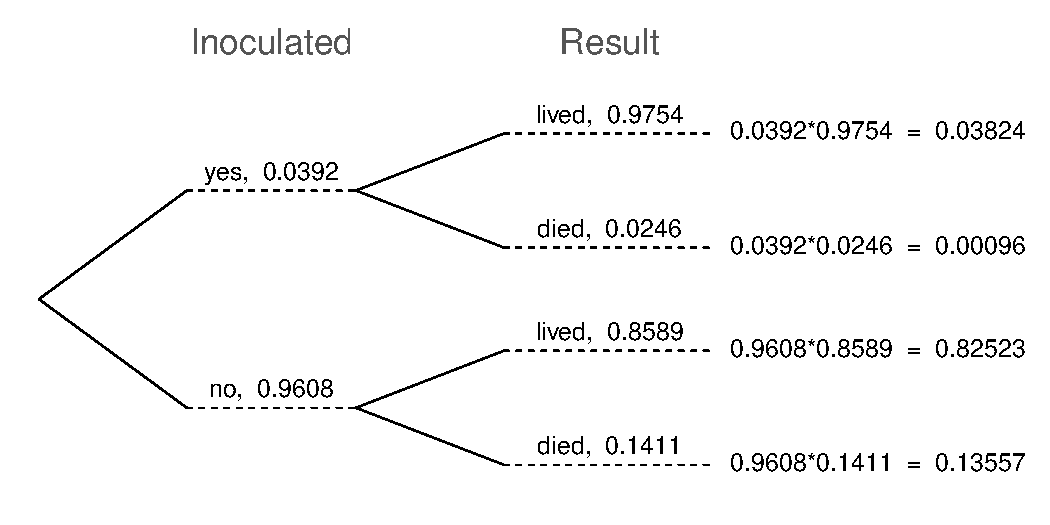
\includegraphics[width=0.93\textwidth]{ch_probability_oi_biostat/figures/smallpoxTreeDiagram/smallpoxTreeDiagram}
\caption{A tree diagram of the \data{smallpox} data set.}
\label{smallpoxTreeDiagram}
\end{figure}

Tree diagrams are annotated with marginal and conditional probabilities, as shown in Figure~\ref{smallpoxTreeDiagram}. This tree diagram splits the smallpox data by \var{inoculation} into the \resp{yes} and \resp{no} groups with respective marginal probabilities 0.0392 and 0.9608. The secondary branches are conditioned on the first, so we assign conditional probabilities to these branches. For example, the top branch in Figure~\ref{smallpoxTreeDiagram} is the probability that \var{result} = \resp{lived} conditioned on the information that \var{inoculated} = \resp{yes}. Joint probabilities can be constructed at the end of each branch in the tree by multiplying the numbers from left to right. These joint probabilities are computed using the General Multiplication Rule:
\begin{eqnarray*}
&& P(\text{\var{inoculated} = \resp{yes} and \var{result} = \resp{lived}}) \\
	&&\quad = P(\text{\var{inoculated} = \resp{yes}}) P(\text{\var{result} = \resp{lived}}|\text{\var{inoculated} = \resp{yes}}) \\
	&&\quad = (0.0392) (0.9754) =0.0382
\end{eqnarray*}


In addition to being a graphical representation of how to compute a probability, tree diagrams are a useful way to organize the information in a probability problem and can often reduce a seemingly difficult problem to a series of simple steps

\begin{example}  

In the general population, about 1 in 28 individuals (approximately 3.6\%) is an unaffected carrier of a mutation in the cystic fibrosis gene, \textit{CFTR}, discussed in example~\ref{CFInheritanceExample}.  Most unaffected carriers are unaware that they harbor the mutation.  Suppose that people with cystic fibrosis do not live long enough to reproduce with a partner.  In the absence of any testing information, what is the probability that a child of two parent will have CF?
	
	\textit{DH: solution not given for now, since I did not want to take the time to draw the tree.  This will be a good example to also solve algebraically, to show that the tree diagram is a representation of the theorem of total prob. Useful, since it will come up with Bayes Thm. Borrow some of the wording from the solution to the grade problem in OI that I removed here.  Below has a start of the solution}
	
	
\textit{solution}
The probabilities calculated in example~\ref{CFInheritanceExample} were conditional probabilities given the carrier status of the parents, though that term was not used in the example.  This exercise asks for an unconditional probability about the disease status of the child, with no additional information about the parents.  The solution uses methods already discussed, but combined is a series of steps.  

The main steps are to first enumerate all the possibilities for carrier status of the parents, calculate the probabilities of each of those probabilities, then calculate the conditional probability of an affected child, given each of the possible outcomes of the parents, and finally use a tree to calculate the probability of a child being affected. Since the problem assumes that affected parents do not reproduce, the pair of parents must satisfy one of the events $A$ = (neither parent is a carrier), $B$ (the mother is a carrier, the father is not), $C$ = (the father is a carrier, the mother is not), $D$ = (both parents are carriers). Since the carrier status of the mother is independent of that of the father, the probabilities of these events are:

\begin{itemize}
	\item $P(A) = (1 - 0.036)(1 - 0.036) = 0.929$
	
	\item $P(B) = P(C) = (1 - 0.036)(0.036) = 0.035$
	
	\item $P(D) = (0.036)(0.036) = 0.001$
\end{itemize}
	
These probabilities do not sum to one because the events where one or both parents are homozygous for the mutation, that is, are affected.

\textit{DH: solution continues now with the conditional probabilities and the tree.  We should think about whether this example is too big of a step from the others, and perhaps add an intermediate example}

\textit{JV: I agree that this might be too much at once... }

\end{example}

\end{comment}
\subsection{Bayes' Theorem}
\label{bayesTheoremSubsection}

\index{Bayes' Theorem|(}

This chapter began with a straightforward question -- what are the chances that a woman with an abnormal (i.e., positive) mammogram has breast cancer?  For a clinician, this question can be rephrased as the conditional probability  that a woman has breast cancer, given that her mammogram is abnormal. This conditional probability is called the \term{positive predictive value} of a mammogram.  

The characteristics of a mammogram (and diagnostic tests in general) are given with the reverse conditional probabilities --  the probability that if a woman in fact has breast cancer, a mammogram will detect it.  More concisely, if $A = \text{\{a mammogram is  positive\}}$ and $B = \text{\{a woman has breast cancer\}}$, the first question is answered by finding $P(A|B)$, while the the known characteristics of a mammogram specify $P(B|A)$.

This type of problem arises so often in medicine that is useful to have several strategies to approach the problem -- 1) constructing tree diagrams, 2) using a purely algebraic approach using Bayes' Theorem, and 3) creating contingency tables based on calculating conditional probabilities from a large, hypothetical population.

\begin{example}{In Canada, about 0.35\% of women over 40 will develop breast cancer in any given year. A common screening test for cancer is the mammogram, but it is not perfect. In about 11\% of patients with breast cancer, the test gives a \term{false negative}: it indicates a woman does not have breast cancer when she does have breast cancer. Similarly, the test gives a \term{false positive} in 7\% of patients who do not have breast cancer: it indicates these patients have breast cancer when they actually do not.\footnote{The probabilities reported here were obtained using studies reported at \oiRedirect{textbook-breastCancerDotOrg_20090831b}{www.breastcancer.org} and \oiRedirect{textbook-ncbi_nih_breast_cancer}{www.ncbi.nlm.nih.gov/pmc/articles/PMC1173421}.} If a random selected woman over 40 is tested for breast cancer using a mammogram and the test is positive -- that is, the test suggests the woman has cancer -- what is the probability she has breast cancer?}
\label{probabilityOfBreastCancerGivenPositiveTestExample}
\end{example}

\subsubsection{Solution 1. Tree Diagram.}

\begin{figure}[h]
	\centering
	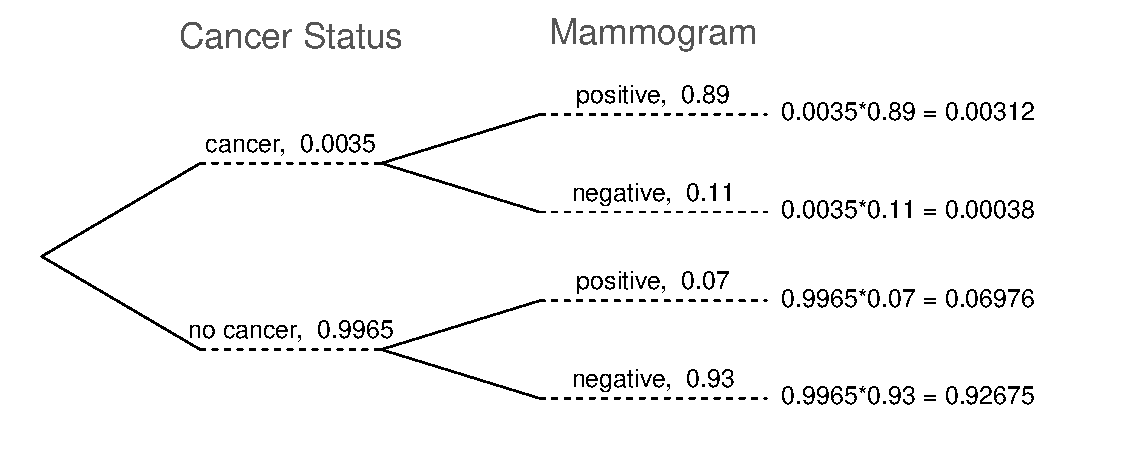
\includegraphics[width=0.93\textwidth]{ch_probability_oi_biostat/figures/BreastCancerTreeDiagram/BreastCancerTreeDiagram}
	\caption{A tree diagram for breast cancer screening.}
	\label{BreastCancerTreeDiagram}
\end{figure}

A \term{tree diagram} is a tool to organize outcomes and probabilities around the structure of data, and is especially useful when two or more processes occur in a sequence, with each process is conditioned on its predecessors. For this problem, the population can first be split by cancer status: \texttt{cancer} or \texttt{no cancer}. Following this split, mammogram results can be either \texttt{positive} or \texttt{negative}. As shown in Figure~\ref{BreastCancerTreeDiagram}, the primary branch shows the marginal probabilities 0.0035 and 0.9965. 

The secondary branches are conditioned on the primary branch and show conditional probabilities; for example, the top branch is the probability that a mammogram is positive given that an individual has cancer. The problem provides enough information to compute the probability of testing positive if breast cancer is present ($1.00 - 0.11=0.89$). 

Joint probabilities can be constructed at the end of each branch by multiplying the numbers from left to right, such as the probability that a woman tests positive given that she has breast cancer (abbreviated as BC):

\begin{align*}
P(\text{BC and mammogram$^+$}) &= P(\text{mammogram$^+$ } |\ \text{BC})  P(\text{BC}) \\
	&= (0.89) (0.0035) = 0.00312
\end{align*}

Using the tree diagram allows for the information in the problem to be mapped out in a way that makes it easier to see how the desired conditional probability can be calculated. In this case, the diagram makes it clear that there are two scenarios in which someone can test positive: either testing positive when having breast cancer or by testing positive in the absence of breast cancer. To find the probability that someone has breast cancer given that they test positive, apply the conditional probability formula: divide the probability of testing positive when having breast cancer by the probability of testing positive.

The probability of a positive test result is the sum of the two corresponding scenarios:
\begin{align*}
P(\text{mammogram$^+$}) =&  P(\text{mammogram$^+$ and has BC}) + P(\text{mammogram$^+$ and no BC}) \\
=&P(\text{mammogram$^+$ } | \text{ has BC}) P(\text{has BC}) + P(\text{mammogram$^+$ } | \text{ no BC}) P(\text{no BC}) \\
=& (0.0035)(0.89) + (0.9965)(0.07) = 0.07288
\end{align*}

Thus, if the mammogram screening is positive for a patient, the probability that the patient has breast cancer is given by: 
\begin{align*}
P(\text{has BC } | \text{ mammogram$^+$})
	&= \frac{P(\text{has BC and mammogram$^+$})}{P(\text{mammogram$^+$})}\\
	&= \frac{0.00312}{0.07288} \approx 0.0428
\end{align*}

Even with a positive mammogram, there is still only a~4\%~chance of breast cancer!   

%DH: \textit{DH: return to this to finish why low prevalence leads to low ppv. that is the important concept for pre-meds and others}

\subsubsection{Solution 2. Bayes' Rule.}

The process used to solve the problem via the tree diagram can be condensed into a single algebraic expression by substituting the original probability expressions into the numerator and denominator:

\begin{small}
\begin{align*}
P(\text{has BC } | \text{ mammogram$^+$})
&= \frac{P(\text{has BC and mammogram$^+$})}{P(\text{mammogram$^+$})} \\
&= \frac{P(\text{mammogram$^+$ } | \text{ has BC})  P(\text{has BC})}
{[P(\text{mammogram$^+$ } | \text{ no BC}) P(\text{no BC})] + [P(\text{mammogram$^+$ } | \text{ has BC}) P(\text{has BC})]}
\end{align*}
\end{small}

The generalization of this formula is known as Bayes' Theorem or Bayes' Rule.

\begin{termBox}{\tBoxTitle{Bayes' Theorem}
Consider the following conditional probability for variable 1 and variable 2:\vspace{-1.5mm}
\begin{align*}
P(\text{outcome $A_1$ of variable 1 } | \text{ outcome $B$ of variable 2})
\end{align*}
Bayes' Theorem states that this conditional probability can be identified as the following fraction:\vspace{-1.5mm}
\begin{align}
\frac{P(B | A_1) P(A_1)}
	{P(B | A_1) P(A_1) + P(B | A_2) P(A_2) + \cdots + P(B | A_k) P(A_k)}
	\label{equationOfBayesTheorem}
\end{align}
where $A_2$, $A_3$, ..., and $A_k$ represent all other possible outcomes of the first variable.}\index{Bayes' Theorem|textbf}
\end{termBox}

The numerator identifies the probability of getting both $A_1$ and $B$. The denominator is the marginal probability of getting $B$. This bottom component of the fraction appears describes the adding of probabilities from the different ways to get $B$. 

To apply Bayes' Theorem correctly, there are two preparatory steps:
\begin{enumerate}
\setlength{\itemsep}{0mm}
\item[(1)] First identify the marginal probabilities of each possible outcome of the first variable: $P(A_1)$, $P(A_2)$, ..., $P(A_k)$.
\item[(2)] Then identify the probability of the outcome $B$, conditioned on each possible scenario for the first variable: $P(B | A_1)$, $P(B | A_2)$, ..., $P(B | A_k)$.
\end{enumerate}
Once each of these probabilities are identified, they can be applied directly within the formula.

\subsubsection{Solution 3. Contingency Table.}

\textit{JV: Leaving this empty for now...}

%%%%%
%
% revisions to here 14sep2015 11:36.  Not satisfied with the treatment of BR here, and we need more examples


% index commands below should be inserted just before section on sampling from a small population

\index{Bayes' Theorem|)}
\index{tree diagram|)}
\index{conditional probability|)}
\index{probability|)}


\textC{\newpage}



%_________________
\section{Random variables}
\label{randomVariablesSection}

\index{random variable|(}

When planning clinical research studies, investigators try to anticipate the results they might see under certain hypotheses. The treatments for some forms of cancer, such as advanced lung cancer, are only effective in a small percentage of patients (typically 20\% or less). When planning a study of a new drug for advanced cancer, it is useful to ask what the expected outcome might be if, for instance, 20\% of patients have a good response (a relatively unsuccessful treatment) or 50\% do (a potentially useful drug).  In a study with 20 participants, one would expect 4 participants to have a good response if the drug does not look promising, and 10 if the drug seemed potentially effective. Other numbers of good responses would be expected for treatments that were either more or less successful than the ones in this example. 

The anticipated outcome in this hypothetical study is an example of a \term{random variable}: something that measures the outcome numerically and seems random because it is not observed before the study is conducted. Since random variables provide mathematical models for data before it has been observed, they are useful in many applications of statistics. Random variables can be used to model more than just the expected outcome of a study. Under the working assumption that 20\% of patients will typically respond to a treatment, investigators would expect 4 responses on average, and not be surprised to see 3 or 5. However, they might be surprised to see 12 or more responses; random variables provide a tool for calculating precisely how unlikely such a result might be.

This section outlines some general concepts used with random variables, while Chapter 3 explores specific types of random variables.


\subsection{Distributions of Random Variables}

Formally, a random variable assigns numerical values to the outcome of a random phenomenon, and is usually written with a capital letter such as $X$, $Y$, or $Z$. 

If a coin is tossed three times, the outcome is the sequence of observed heads and tails. One such outcome might be TTH: tails on the first two tosses, heads on the third. If the random variable $X$ is the number of heads for the three tosses, $X=1$; if $Y$ is the number of tails, then $Y=2$. For the sequence THT, only the order has changed, but the values of $X$ and $Y$ remain the same. For the sequence HHH, however, $X=3$ and $Y=0$. Even in this simple setting, is possible to define other random variables; for example, if $Z$ is the toss when the first H occurs, then $Z=3$ for the first set of tosses (TTH) and 1 for the third set (HHH).  

\begin{figure}[h]
	\centering
	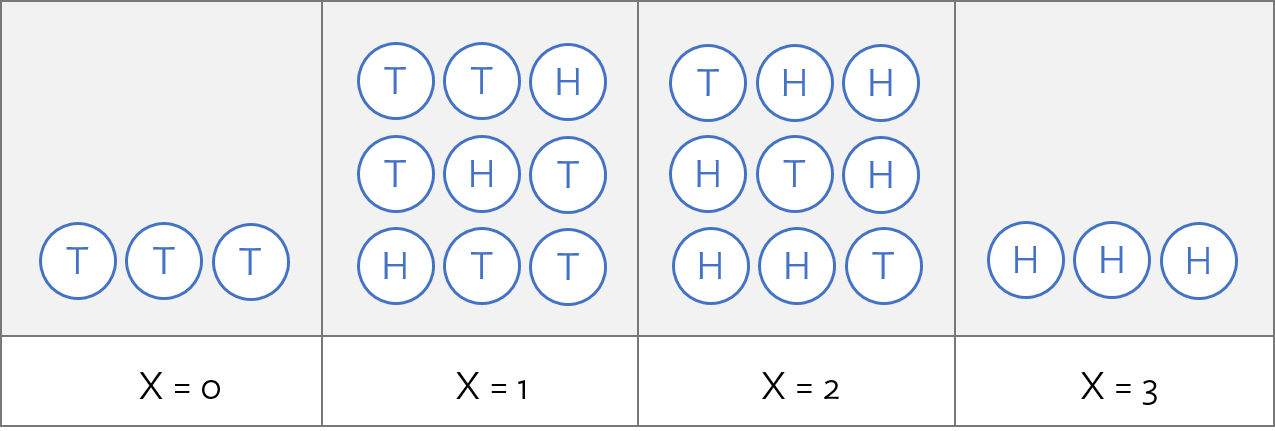
\includegraphics[width=0.70\textwidth]
	{ch_probability_oi_biostat/figures/coinToss/coinToss.png}
	\caption{Possible outcomes for tossing a coin three times}
	\label{coinToss}
\end{figure}

If probabilities can be assigned to the outcomes in a random phenomenon or study, then those can be used to assign probabilities to values of a random variable.  Using independence, $P(\text{HHH}) = (1/2)^3 = 1/8$.  Since $X$ in the above example can only be three if the three tosses are all heads, $P(X=3) = 1/8$.  The distribution of a random variable is the collection of probabilities for all of the variable's unique values. Figure~\ref{coinToss} shows the eight possible outcomes when a coin is cossed three times: TTT, HTT, THT, TTH, HHT, HTH, THH, HHH. The variable $X = 0$ for the first set of tosses, $X = 1$ for the next three, $X = 2$ for the following three, and $X = 3$ for the last set (HHH).  

Using independence again, each of the 8 outcomes have probability 1/8, so $P(X = 0) = P(X = 3) = 1/8$ and $P(X = 1) = P(X = 2) = 3/8$. For random variables with a small number of outcomes, it is often easier and more instructive to display its distribution in a table. Table~\ref{distCoinTossing} shows the probability distribution for $X$.  Probability distributions for random variables follow the rules for probability; for instance, the sum of the probabilities must be 1.00.  The possible outcomes of $X$ are labeled with a corresponding lower case letter $x$ and subscripts.  The values of X are $x_1=0$, $x_2=1$,  $x_3 = 2$, and $x_4 = 3$; these occur with probabilities $1/8$, $3/8$, $3/8$ and $1/8$.

\begin{table}[h]
	\centering 
	\begin{tabular}{l rrrr l}
		\hline 
		$i$ & 1 & 2 & 3 & 4 & Total\\
		\hline
		$x_i$ & 0 & 1 & 2 & 3 & --\\
		$P(X = x_i)$ & 1/8 & 3/8 & 3/8 & 1/8 & 8/8 = 1.00\\
	\end{tabular}
	\caption{Tabular form for the distribution of the number of heads in three coin tosses}
	\label{distCoinTossing}
\end{table}

\begin{figure}[h]
\centering
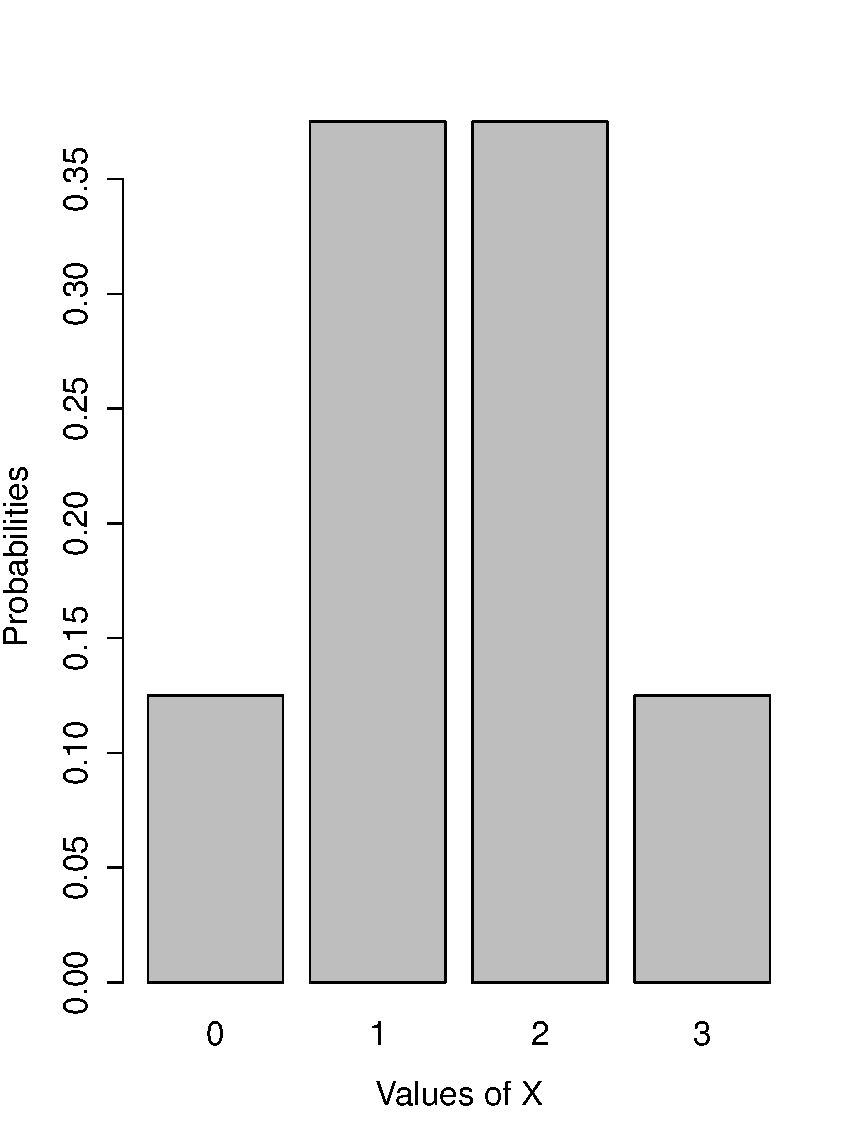
\includegraphics[width=0.7\textwidth]
{ch_probability_oi_biostat/figures/barPlotCoinTossing/barPlotCoinTossing.pdf}
\caption{Bar plot of the distribution of the number of heads in three coin tosses }
\label{barPlotCoinTossing}
\end{figure}

Bar graphs can be used to show the distribution of a random variable.  Figure~\ref{barPlotCoinTossing} is a bar graph of the distribution of $X$ in the coin tossing example. When bar graphs are used to show the distribution of a dataset, the heights of the bars show the frequency of observations; bar heights showing a probability distribution show the probabilities of possible values of a random variable.

$X$ is an example of a \term{discrete random variable} since it takes on a finite number of values.\footnote{Some discrete random variables have an infinite number of possible values, such as all the non-negative integers.}  Because $X$ arises in a simple experiment (3 tosses of a coin) in which probabilities are easy to calculate, calculating the probability distribution of $X$ is straightforward and the bar plot is not particularly informative.  

The hypothetical clinical study at the beginning of this section raised the question of how surprising it would be to observe 12 or more responses out of 20 in a setting where only 20\% of patients are expected to respond to treatment.  Suppose $X$ is a random variable that will denote the possible number of responding participants in a clinical study. $X$ will have the same probability distribution as the number of heads in 20 tosses of a weighted coin, where the probability of landing heads is 0.2 instead of $1/2 = 0.5$.  The graph of the probability distribution for $X$ in Figure~\ref{distRespClinStudy} can be used to approximate this probability.\footnote{This and other useful distributions will be examined in detail in Chapter 3} The nine values (12, 13,\ldots, 20) make up the event 12 or more, and the graph shows that each of these probabilities is smaller than 0.005, so the chance of 12 or more responses is less than 0.01, or clearly less than 1\%.  Formulas in Chapter 3 can be used to show that the exact probability is slightly larger than 0.0001.

\begin{figure}[h]
\centering
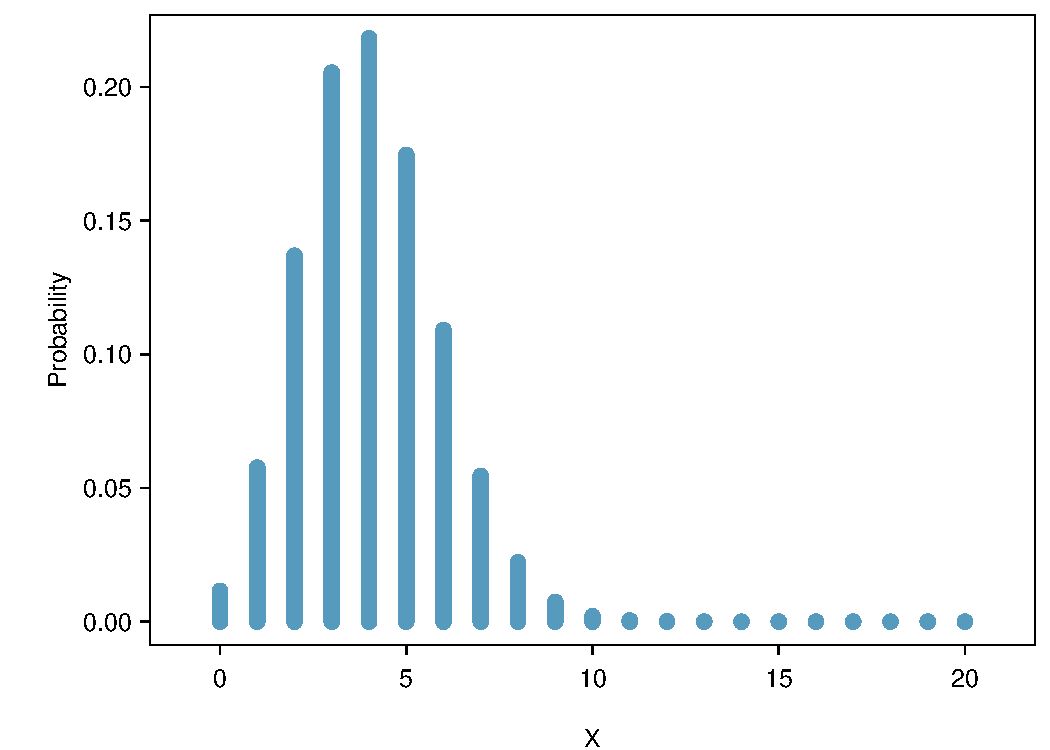
\includegraphics[width=0.70\textwidth]
{ch_probability_oi_biostat/figures/distRespClinStudy/distRespClinStudy.pdf}
\caption{Bar plot of the distribution of the number of responses in a study with 20 participants and response probability 0.20}
\label{distRespClinStudy}
\end{figure}

%DH:  \textit{DH: this example can be improved, and the graph could be improved as well.}


\subsection{Expectation}

\index{expectation|(}

Just like distributions of data, distributions of random variables also have means, variances, standard deviations, medians, etc.; these characteristics are computed a bit differently for random variables. To calculate the mean of a random variable, multiply each possible value by its corresponding probability and add these products. The mean of a random variable is called its \term{expected value} and written $E(X)$ -- it is the value one would expect to see if the variable were to be observed. For the variable $X$ in the last section:

\begin{align*}
E(X) &= (0)(P(X=0)) + (1)(P(X=1)) + (2)(P(X=2)) + (3)(P(X = 3)) \\
	&= (0)(1/8) + (1)(3/8) + (2)(3/8) + (3)(1/8) = 12/8 = 1.5
\end{align*}

\begin{termBox}{\tBoxTitle{Expected value of a discrete random variable}
If $X$ takes on outcomes $x_1$, ..., $x_k$ with probabilities $P(X=x_1)$, ..., $P(X=x_k)$, the expected value of $X$ is the sum of each outcome multiplied by its corresponding probability:
\begin{align}
E(X) 	&= x_1 P(X=x_1) + \cdots + x_k P(X=x_k) \notag \\
	&= \sum_{i=1}^{k}x_iP(X=x_i)
\end{align}
The Greek letter $\mu$\index{Greek!mu ($\mu$)} may be used in place of the notation $E(X)$.}
\end{termBox}
The expected value for a random variable represents the average outcome. For example, $E(X)=1.5$ represents the average number of heads in three tosses of a coin, if the three tosses were repeated many times; this is also written as $\mu=1.5$.  It often happens with discrete random variables that the expected value is not precisely one of the possible outcomes of the variable.

\begin{comment}
The expected value of a random variable has the same interpretation as a mean in a dataset. The distribution can be represented by a series of weights at each outcome, and the mean represents the balancing point.
\end{comment}

%DH: \textit{DH: I have omitted the material on continuous distributions and may re-insert it later. I also did not include figure 2.22 from OI, which I like.  Maybe we should put that back as well.} 

%JV: \textit{JV: I'm not as much a fan of that figure. I think the physical interpretation worked better for the initial introduction of a mean, but then here, the idea of an "expected value" is already a clear interpretation.}

\index{expectation|)}

\subsection{Variability in random variables}

How variable will the outcomes be when tossing a coin three times?  The \indexthis{variance}{variance} and \indexthis{standard deviation}{standard deviation} can be used to describe the variability of a random variable. Section~\ref{variability}
introduced a method for finding the variance and standard deviation for a dataset.  Deviations from the mean ($x_i - \mu$) were squared, then averaged to compute the variance. In the case of a random variable, squared deviations are again used, this time deviations from the mean of the random variable, and their sum is weighted by the corresponding probabilities. This weighted sum of squared deviations equals the variance, and the standard deviation is again the square root of the variance, just as in Section~\ref{variability}.

\begin{termBox}{\tBoxTitle{General variance formula}
If $X$ takes on outcomes $x_1$, ..., $x_k$ with probabilities $P(X=x_1)$, ..., $P(X=x_k)$ and expected value $\mu=E(X)$, then the variance of $X$, denoted by $\text{Var}(X)$ or the symbol $\sigma^2$, is
\begin{align}
\sigma^2 &= (x_1-\mu)^2 P(X=x_1) + \cdots \notag \\
	& \qquad\quad\cdots+ (x_k-\mu)^2 P(X=x_k) \notag \\
	&= \sum_{j=1}^{k} (x_j - \mu)^2 P(X=x_j)
\end{align}
The standard deviation of $X$, labeled $\sigma$\index{Greek!sigma ($\sigma$)}, is the square root of the variance.}
\end{termBox}
\marginpar[\raggedright\vspace{-47mm}

$\text{Var}(X)$\vspace{1mm}\\\footnotesize Variance\\of $X$]{\raggedright\vspace{-47mm}

$\text{Var}(X)$\vspace{1mm}\\\footnotesize Variance\\of $X$}

The weighted sum in variance of a random variable can be interpreted as the expectation of the terms $(x_i - \mu)^2$ (instead of just $x_i$), so a compact form for the formula is 
\begin{align*}
	 \sigma_X^2 = E(X - \mu)^2.
\end{align*}

This compact form is not useful for direct computation, but it is useful for understanding the general concept. 

\begin{example}{Compute the variance and standard deviation of $X$, the number of heads in three tosses of a coin.}
    
    In the formula for the variance, $k = 4$ and $\mu_X = E(X) = 1.5$, the variance will be 
    \begin{align}
    \sigma_X^2 &= (x_i-\mu_X)^2P(X=x_1) + \cdots \notag \\
    	& \qquad\quad\cdots+ (x_4-\mu)^2 P(X=x_4) \notag \\
    	&= (0- 1.5)^2(1/8) + (1 - 1.5)^2 (3/8) + 
        (2 -1.5)^2 (3/8) + (3-1.5)^2 (1/8) \notag \\
        &= 3/4 = 0.75.
    \end{align}
    
The standard deviation is $\sqrt{3/4} = \sqrt{3}/2 = 0.866$.  

\end{example}

The coin tossing scenario provides a simple illustration of the mean and variance of a random variable, but it is artificial. 

 \label{healthCareCostsEmployee}
In most typical health insurance plans in the United States, members of the plan pay annually in three categories: a monthly premium, ``out-of-pocket'' costs which include co-payments for each physician visit or prescription, and a deductible amount that members pay each year before the insurance covers service.\footnote{The deductible also includes care and supplies that are not covered by insurance.} Picking a new health plan involves estimating costs for the next year based on a person's best guess at the type and number of services that will be needed.
	
In 2015, Harvard University offered several alternative plans to its employees.   In the Health Maintenance Organization (HMO) plan for employees earning less than \$70,000 per year, the monthly premium was \$79, and the co-payment for each office visit or physical therapy session was \$20. A new employee examined her health records for the last 10 years, and noticed that in three of the 10 years her only office visit was one annual physical.  In four of the 10 years she visited her physician three times, once for a physical, and twice for a cases of the flu. In two years, she had four visits.  In one of the 10 years, she experienced a knee injury that required 3 office visits and 5 physical therapy sessions.

\begin{example} {Ignoring the cost of prescription drugs, over-the-counter medications and the annual deductible amount, what is the expected annual healthcare cost for this employee under the Harvard plan?}  

Let the random variable $X$ denote annual healthcare costs.  It is best to summarize the information in the problem in a table that can also be used for computing the mean and variance of $X$.  If the  last ten years are an accurate picture of annual costs for this employee, $X$ will have four possible values that correspond to the annual cost of the monthly premium plus the visit costs for the four patterns of visits.  The cost of the premium is (12)(\$79) = \$948. The cost of the visits is \$20 times the number of visits.  The values of $X$ are ordered according to increasing numbers of visits. 

For example, the first column in the table contains information about the years in which the employee had one office visit. Adding the \$948 for the annual premium and \$20 for one visit results in $x_{1}=\$968$; $P(X=x_{i}) = 3/10 = 0.30$.

\begin{center}
\begin{tabular}{l rrrr r}
\hline
$i$ & 1 & 2 & 3 & 4 & Total \\
\hline
Number of visits & 1 & 3 & 4 & 8 &\\
$x_i$ & 968 & 1008 & 1028 & 1108 &  \\
$P(X=x_i)$ & 0.30 & 0.40 & 0.20 & 0.10 & 1.0 \\
$x_i P(X=x_i)$ & 290.40 & 403.20 & 205.60 & 110.80 & 1010.00 \\
\hline
\end{tabular}
\end{center}
The expected cost of health care for a year is $\mu=\$1010.00$. The variance can be calculated by extending the table:
\begin{center}
\begin{tabular}{l rrrr r}
\hline
$i$ & 1 & 2 & 3 & 4 & Total \\
\hline
Number of visits & 1 & 3 & 4 & 8 &\\
$x_i$ & 968 & 1008 & 1028 & 1108 &  \\
$P(X=x_i)$ & 0.30 & 0.40 & 0.20 & 0.10 & 1.0 \\
$(x_i)P(X=x_i)$ & 290.40 & 403.20 & 205.60 & 110.80 & 1010.00 \\
$x_i - \mu$ & -42.00  & -2.00  & 18.00  & 98.00 & \\
$(x_i - \mu)^2$ &  1764.00 & 4.00  & 324.00  & 9604 & \\
$(x_i - \mu)^2 P(X=x_i)$ & 529.20  & 1.60  & 64.80  & 960.40 & 1556.00\\
\hline
\end{tabular}
\end{center}
The variance of $X$ is $\sigma^2 = \$1556.00$, and the standard deviation is $\sigma = \$39.45$.  The standard deviation always has the same units as the original measurements. 

\end{example}

%DH: \textit{DH: This problem has potential for the exercises, either by making it more complicated (considering deductibles, etc, or by comparing the mean and standard deviation of two health plans). JV: I like this example.}

\subsection{Linear combinations of random variables}

Sums of random variables arise naturally in many problems. In the health insurance example, the amount spent by the employee during her next five years of employment can be represented as $X_1 + X_2 + X_3 + X_4 + X_5$, where $X_1$ is the cost of the first year, $X_2$ the second year, etc. If the employee's domestic partner also has health insurance with another employer, the total annual cost to the couple would be the sum of the costs for the employee ($X$) and her partner ($Y$), or $X + Y$. In each of these examples, it is intuitively clear that the average cost would be the sum of the average of each term.

Sums of random variables are special cases of linear combinations of variables.  

\begin{termBox}{\tBoxTitle{Linear combinations of random variables and their expected values}
If $X$ and $Y$ are random variables, then a linear combination of the random variables is given by
\begin{align}\label{linComboOfRandomVariablesXAndY}
aX + bY
\end{align}
where $a$ and $b$ are constants.  The mean of a linear combination of random variables is 
\begin{align*}
 E(aX + bY) = aE(X) + bE(Y) = a\mu_X + b\mu_Y
\end{align*}}
\end{termBox}

There are a few special cases of this formula which are especially useful. The formula implies that $E(a + Y) = a + E(Y)$.  This could have been used when calculating the average health costs for the employee by defining $a$ as the fixed cost of the premium ($a=\$948$), and taking $Y$ to be just the cost of the physician visits. Thus, the total annual cost for a year could be calculated as: $E(a + Y) = a + E(Y) = \$948 + E(Y) = \$948 + .30(1 \times \$20) + .40(3 \times \$20) + .20(4 \times \$20) + .10(8 \times \$20)= \$1,010.00$. 

The formula easily generalizes to a sum of any number of random variables. For example, the average health care cost for 5 years (given that the cost for services remains the same) would be: 

\begin{align*}
	E(X_1 + X_2 + X_3 + X_4 + X_5) &= E(X_1) + E(X_2) + E(X_3) + E(X_4) + E(X_5) \\
	         &= 5E(X_1) \\
			 &=(5)(1010) = \$5,050
\end{align*}

\begin{exercise} \label{healthCareCostsPartner}
	Suppose the employee will begin a domestic partnership in the next year, and while she and her companion will begin living together and sharing expenses, she and her partner will keep their existing health insurance plans; both, in fact have the same plan from the same employer.  In the last five years, her new partner visited a physician only once in four of the ten years, and twice in the other six years.   Calculate the expected total cost of health insurance to the couple in the next year.\footnote{Let $X$ represent the costs for the employee and $Y$ represent the costs for her partner. $E(X) = \$1,010.00$, as previously calculated. $E(Y) = 948 + .4(1 \times \$20) + .6(2 \times \$20) = \$980.00$. Thus, $E(X + Y) = E(X) + E(Y) = \$1,010.00 + \$980.00 = \$1,990.00$.}
\end{exercise}

The employee and her partner would also like to know how variable their health care costs would be for the next year.  Calculating the variance and standard deviation of a linear combination of random variables requires more care.  The formula given here requires that the random variables in the linear combination be independent, so that an observation on one of the variables provides no information about the value of the other variable.  With that assumption, the following formula can be used:

\begin{termBox}{\tBoxTitle{Variability of linear combinations of random variables}
The variance of a linear combination of random variables may be computed by squaring the constants, substituting in the variances for the random variables, and computing the result:
\begin{align*}
\text{Var}(aX + bY) = a^2 \text{Var}(X) + b^2\text{Var}(Y)
\end{align*}
This equation is valid as long as the random variables are independent of each other. The standard deviation of the linear combination can be found by taking the square root of the variance.}
\end{termBox}

To calculate the variance and standard deviation for the next year health care costs for the two partners:

\textit{Solution to be added. Start with X = costs for employee and Y the costs for partner, use formula for Var(X + Y). Add the question about whether independence assumption is reasonable.}

The example of health insurance costs has been simplified to make the calculations clearer.  It ignores the fact that many plans have a deductible amount, and that plan members pay for services at different rates before and after the deductible has been reached. Often, insured individuals do not pay for services at all once a maximum amount has been reached in a year. The example also assumes that the proportions of number of physician visits per year, estimated from the last 10 years, can be treated as probabilities measured without error.  Had a different time-span been chosen, the proportions might well have been different.  

\begin{exercise}  The Association of American Medical Colleges (AAMC) introduced a new version of the Medical College Admission Test (MCAT) in the spring of 2015. Data from the scores were recently released by AAMC.\footnote{https://www.aamc.org/students/download/434504/data/percentilenewmcat.pdf}  The test consists of 4 components: chemical and physical foundations of biological systems; critical analysis and reasoning skills; biological and biochemical foundations of living systems; psychological, social and biological foundations of behavior. The overall score is the sum of the individual component scores. The grading for each of the four components is scaled so that the mean score is 125.  The means and standard deviations for the four components and the total scores for the population taking the exam in May 2015 exam are shown in table~\ref{table:mcatScoreDistribution}.
	
Show that the standard deviation in the table for the total score does not agree with that obtained using the formula for the standard deviation of the sum of random variables.  Why do you think that is the case?

	\begin{table}[h]
		\centering
		\begin{tabular}{lrr}
			\hline
			\textbf{Component} & \textbf{Mean} & \textbf{Standard Deviation}\\
			\hline
			             Chem. Phys. Found. &   125 &   3.0\\
			             Crit. Analysis &   125 &    3.0 \\
			             Living  Systems &  125 &     3.0\\
			             Found. Behavior&   125 &     3.1\\
			             \textbf{Total} &    500 &     10.6\\
			\hline
		\end{tabular}
		\caption{Means and Standard Deviations for MCAT Scores}
		\label{table:mcatScoreDistribution}
	\end{table}	
\end{exercise}

\textit{Solution to be added, but only as far as noting that independence is not likely to be true. Begin by applying the formula that assumes independence.}


\section{Distributions for pairs of random variables (special topic)}

\index{joint distribution for random variables|(}
\index{marginal distribution for random variables|(}

The summary MCAT score is more variable than implied by the formula for computing the standard deviation for sums of random variables because the component scores are not independent, but correlated. Individuals scoring well on one component of the exam are likely to score well on other parts.  When two random variables tend to vary together, they are called \term{correlated random variables}.  There are many examples of correlated random variables, including height and weight in a population of individuals, the scores of verbal and quantitative SAT exams, and gestational age and birth weight of newborns.  When two random variables $X$ and $Y$ are correlated,
\begin{equation*} 
	\text{Variance}(X + Y) = \text{Variance}(X) + \text{Variance}(Y) + 
	2 \sigma_X \sigma_Y\text{Correlation}(X,Y) 
	\label{eq:generalVarianceSumRVs}
\end{equation*}
and
\begin{equation*}
	\text{Variance}(X - Y) = \text{Variance}(X) + \text{Variance}(Y) - 
	2 \sigma_X \sigma_Y\text{Correlation}(X,Y) 
	\label{eq:generalVarianceDiffRVs}
\end{equation*}
The standard deviation for the sum or difference will be the square root of the variance.

Correlation between random variables is similar to correlation between pairs of observations in a dataset, with some important differences.  Calculating a correlation $r$ in a dataset was introduced in Section~\ref{scatterPlots} and uses the formula 
\begin{align*}
      r &=  \frac{1}{n-1}\sum^{n}_{i=1}
      \left(\frac{x_{i}-\overline{x}}
      {s_{x}}\right)\left(\frac{y_{i}-\overline{y}}{s_{y}}\right)
\end{align*} 
The correlation coefficient $r$ is an average of products, with each term in the product measuring the distance between $x$ and its mean $\overline{x}$ or $y$ and its mean $\overline{y}$, after the distances have been scaled by respective standard deviations.

The compact formula for the correlation between two random variables $X$ and $Y$  uses the same idea; it is given by
\begin{equation*}
	\rho_{X,Y} = E\left(\frac{X - \mu_x}{\sigma_X}\right)\left(\frac{Y - \mu_Y}{\sigma_Y} \right),
	\label{eq:generalFormulaCorrelation}
\end{equation*}
where $\rho_{X,Y}$ is the correlation between the two variables, and $\mu_X, \mu_Y$, $\sigma_X, \sigma_Y$ are the respective means and standard deviations for $X$ and $Y$. Just as with the mean of a random variable, the expectation in the formula for correlation is a weighted sum of products, with with each term weighted by the probability of values for the pair $(X,Y)$.  Equation~\ref{eq:generalFormulaCorrelation} is useful for understanding analogy between correlation of random variables and observations in a dataset, but it cannot be used to calculate $\rho_{X,Y}$ without the probability weights.  The weights come from the \term{joint distribution} of the pair of variables $(X,Y)$.  Joint probabilities were discussed in section~\ref{marginalAndJointProbabilities}.

\begin{termBox}{\tBoxTitle{Joint distribution}
The \term{joint distribution} for a pair of random variables is the collection of probabilities

\begin{align*}
	  p(x_i,y_j) = P(X=x_i \text{ and } Y = y_j) = P(X=x_i, Y=y_j)
\end{align*}
for all pairs of values $(x_i,y_j)$ for the pair of random variables $(X,Y)$.}
\end{termBox}

Joint distributions quickly become complicated.  If $X$ and $Y$ have $k_1$ and $k_2$ possible values respectively, there will be $(k_1)(k_2)$ possible $(x,y)$ pairs. This is unlike pairs of values $(x,y)$ observed in a dataset, where each observed value of $x$ is usually paired with only one value of $y$. A joint distribution is often best displayed as a table of probabilities, with $(k_1)(k_2)$ entries.  Table~\ref{table:generalJointDistribution} shows the general form of the table. 

\begin{table}[h]
	\caption{Table for a joint distribution. Entries are probabilities for pairs ($x_i, y_j$)}
	\label{table:generalJointDistribution}
	\centering
	\begin{tabular}{ccccc}
		\hline
		& \multicolumn{4}{c}{\textbf{Values of $Y$}} \\
		\hline
		\textbf{Values of $X$} & $y_1$ & $y_2$ & $\cdots$ & $y_{k_2}$ \\
		             $x_1$ &   $p(x_1, y_1)$ &   $p(x_1, y_2)$  & $\cdots$  & $p(x_1, y_{k_2})$  \\
		              $x_2$ &  $p(x_2, y_1)$   &  $p(x_2, y_2)$  & $\cdots$ &   $p(x_2, y_{k_2})$ \\
		             $\vdots$ &   $\cdots$  &  $\cdots$  &  $\cdots$ &   $\cdots$ \\
		              $x_{k_1}$ & $p(x_{k_1}, y_1)$ &  $p(x_{k_1}, y_2)$  &  $\cdots$ & $p(x_{k_1}, y_{k_2})$ \\
		             
	\end{tabular}
\end{table}

\newpage
Previously, the calculation of variability in health care costs for an employee and her partner relied on the assumption that the number of health episodes between the two are independent random variables. It might be reasonable to assume that the health status of one person gives no information about the other's health, given that the two are not related and were not previously living together. However, correlation between random variables can be subtle. For example, couples are often attracted to each other because of common interests or lifestyles, which suggests that health status may not actually be independent.

Might the health care costs for the employee and her domestic partner be correlated? To start, examine the joint distribution of costs by making a table of all possible combinations of costs for the last 10 years (these costs were previously calculated in Example~\ref{healthCareCostsEmployee} and Guided Practice~\ref{healthCareCostsPartner}). Entries in the table are probabilities of pairs of annual costs. For example, the entry 0.25 in the second row and second column of Table~\ref{healthExpensesJointDistribution} indicates that in approximately \%25 of the last 10 years, the employee paid \$1,008 in costs and her partner paid \$988.

\begin{table}[h]
\centering
\begin{tabular}{crr}
  \hline \\
  &   \multicolumn{2}{c}{\textbf{Partner costs}} \\
\textbf{Employee costs} & \textbf{\$968} & \textbf{\$988} \\ 
  \hline
\textbf{\$968} & 0.18 & 0.12 \\ 
 \textbf{\$1,008} & 0.15 & 0.25 \\ 
 \textbf{\$1,028}  & 0.04 & 0.16 \\ 
 \textbf{\$1,108}  & 0.03 & 0.07 \\ 
   \hline
\end{tabular}
\caption{Joint distribution of health care costs.} 
\label{healthExpensesJointDistribution}
\end{table}
% R code for the table is in the chap 2 rcode file, but does not quite produce this table.  Could not get the rownames, colnames to appear

When two variables $X$ and $Y$ have a joint distribution, the marginal distribution of $X$ is the collection of probabilities for $X$ when $Y$ is ignored.  If $X$ represents employee costs and $Y$ represents partner costs, the event $(X = \$968)$ consists of the two  disjoint events $(X = \$968, Y = \$968)$ and $(X = \$968, Y = \$988)$, so $P(X = \$968) = 0.18 + 0.12 = 0.30$, the sum of the first row of the table. 

The row sums in Table~\ref{healthExpensesJointDistribution} are the values of the \term{marginal distribution} of $X$. Similarly, the column sums will be the values of the marginal distribution of $Y$.  The marginal distributions of $X$ and $Y$ are shown in Table ~\ref{healthExpensesJointMarginalDistribution}, along with the joint distribution of $X$ and $Y$.
\newpage

\begin{table}[h]
\centering
\begin{tabular}{crrr}
  \hline \\
  &   \multicolumn{2}{c}{\textbf{Partner Costs}} & \textbf{Marg. Dist.}\\
\textbf{Employee costs} & \textbf{\$968} & \textbf{\$988} & \textbf{Employee Costs} \\ 
  \hline
\textbf{\$968} & 0.18 & 0.12 & 0.30\\ 
 \textbf{\$1,008} & 0.15 & 0.25 & 0.40 \\ 
 \textbf{\$1,028}  & 0.04 & 0.16 & 0.20\\ 
 \textbf{\$1,108}  & 0.03 & 0.07  & 0.10\\ 
   \hline
 \textbf{Marg. Dist.} & 0.40 & 0.60 & 1.00 \\
 \textbf{Partner Costs} &  &  & \\
 \hline \\
\end{tabular}
\caption{Joint and Marginal Distributions of Health Care Costs.} 
\label{healthExpensesJointMarginalDistribution}
\end{table}

\textit{DH: Formatting of table has to be improved}


\begin{example}{Calculate the correlation between employee costs and the standard deviation of the sum of the costs for the couple.}
	
	\textit{Not filling in the details now. Proceeds by showing that the marginal distributions are the same as those used earlier, then calculating $\sigma_X, \sigma_Y$ etc.  Variance using equation~\ref{eq:generalVarianceSumRVs}}
	\end{example}

\textit{Outline for the remainder of this section
	\begin{itemize}[--]
		\item general form of table for joint, marginal distributions
		\item conditional distributions
		\item example
	\end{itemize}}

\index{joint distribution for random variables|)}
\index{marginal distribution for random variables|)}
\index{random variable|)}

\section{Continuous distributions}
\label{contDist}

\index{data!FCID|(}
\index{hollow histogram|(}

Figure~\ref{fdicHistograms} shows a few different hollow histograms of the variable \var{height} for 3 million US adults from the mid-90's.\footnote{This sample can be considered a simple random sample from the US population. It relies on the USDA Food Commodity Intake Database.} Examine the transition from a boxy hollow histogram in the top-left of Figure~\ref{fdicHistograms} to the much smoother plot in the lower-right. In this last plot, the bins are so narrow that the hollow histogram begins to resemble a smooth curve. This suggests that population height, as a continuous numerical variable, might best be explained by a curve that represents the outline of extremely slim bins.

\begin{figure}[h!]
	\centering
	\subfigure[]{
		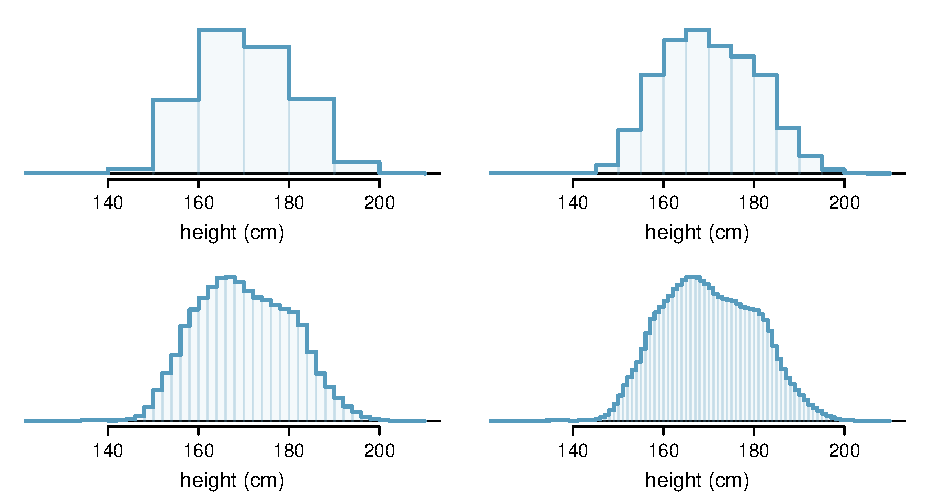
\includegraphics[width=0.70\textwidth]{ch_probability_oi_biostat/figures/fdicHistograms/fdicHistograms}
		\label{fdicHistograms}
	}
	\subfigure[]{
		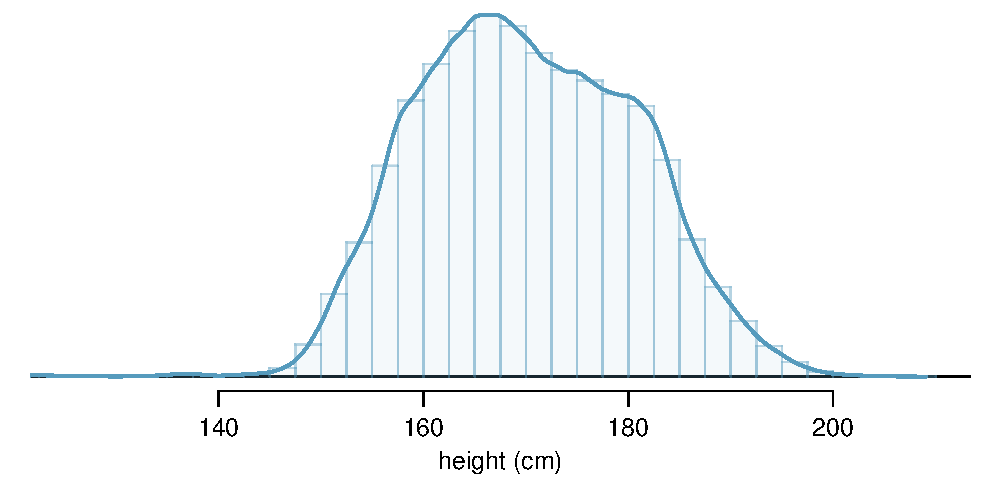
\includegraphics[width=0.70\textwidth]{ch_probability_oi_biostat/figures/fdicHeightContDist/fdicHeightContDist}
		\label{fdicHeightContDist}		
	}
	\caption{\subref{fdicHistograms} Four hollow histograms of US adults heights with varying bin widths. \subref{fdicHeightContDist} The continuous probability distribution of heights for US adults.}
\end{figure}

This smooth curve represents a \term{probability density function} (also called a \term{density} or \term{distribution}), and such a curve is shown in Figure~\ref{fdicHeightContDist} overlaid on a histogram of the sample. A density has a special property: the total area under the density's curve is 1. The distribution of a continuous distribution is specified by a density function instead of a table like the one in Table~\ref{distCoinTossing}.

\index{hollow histogram|)}

\subsection{Probabilities from continuous distributions}

\begin{figure}[h!]
	\centering
	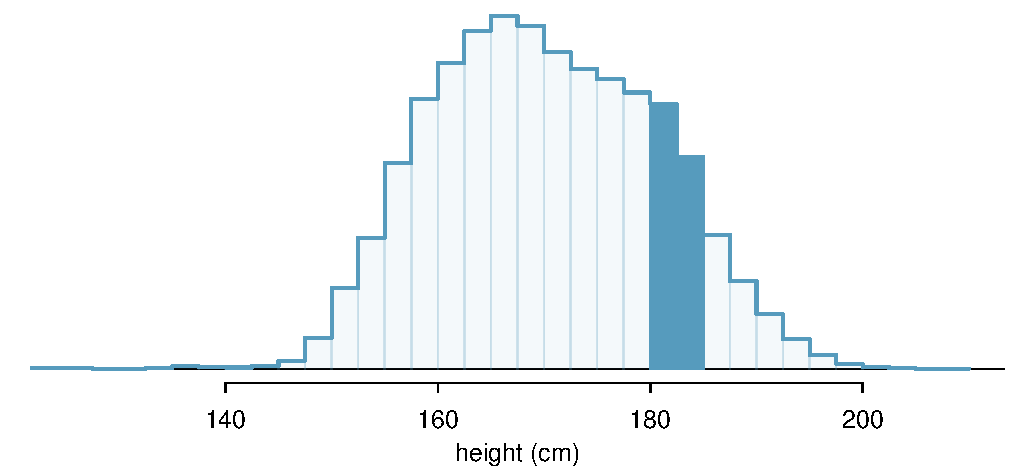
\includegraphics[width=0.7\textwidth]{ch_probability_oi_biostat/figures/usHeightsHist180185/usHeightsHist180185}
	\caption{A histogram with bin sizes of 2.5 cm. The shaded region represents individuals with heights between \resp{180} and \resp{185} cm. }
	\label{usHeightsHist180185}
\end{figure}

\begin{example}{What proportion of the sample is between \resp{180} cm and \resp{185} cm tall (about 5'11" to 6'1"), if the two bins in this region have counts of 195,307 and 156,239 people?}\label{contDistProb}
	
Add the heights of the bins in the range \resp{180} cm and \resp{185} and divide by the sample size:
	\begin{eqnarray*}
		\frac{195,307+156,239}{\text{3,000,000}} = 0.1172
	\end{eqnarray*}
	This fraction is the same as the proportion of the histogram's area that falls in the range \resp{180} to \resp{185} cm.
\end{example}

\begin{figure}
	\centering
	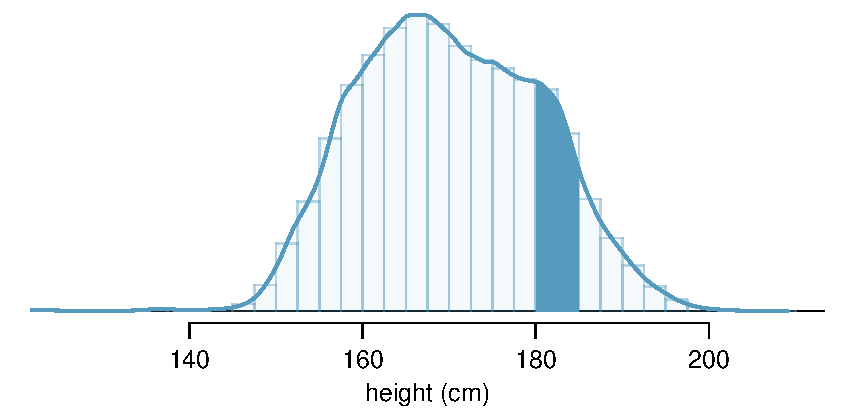
\includegraphics[width=0.7\textwidth]{ch_probability_oi_biostat/figures/fdicHeightContDistFilled/fdicHeightContDistFilled}
	\caption{Density for heights in the US adult population with the area between 180 and 185 cm shaded. Compare this plot with Figure~\ref{usHeightsHist180185}.}
	\label{fdicHeightContDistFilled}
\end{figure}

For a continuous distribution, the probability can be calculated by finding the area of the shaded region under the curve between \resp{180} and \resp{185} (with the help of a computer):

\begin{eqnarray*}
P(\text{\var{height} between \resp{180} and \resp{185}})
	= \text{area between \resp{180} and \resp{185}}
	= 0.1157
\end{eqnarray*}

The probability that a randomly selected person is between \resp{180} and \resp{185} cm is 0.1157. This is very close to the estimate from Example~\ref{contDistProb}: 0.1172. 

\begin{exercise}
Three US adults are randomly selected. The probability a single adult is between \resp{180} and \resp{185} cm is 0.1157.\footnote{(a) Assume independence. $(0.1157)  (0.1157) (0.1157) = 0.0015$. (b) $(1-0.1157)^3 = 0.692$} \vspace{-1.5mm}
\begin{enumerate}
\setlength{\itemsep}{0mm}
\item[(a)] What is the probability that all three are between \resp{180} and \resp{185} cm tall?
\item[(b)] What is the probability that none are between \resp{180} and \resp{185} cm?
\end{enumerate}
\end{exercise}

\begin{example}{What is the probability that a randomly selected person is \textbf{exactly} \resp{180}~cm? Assume you can measure perfectly.}
\label{probabilityOfExactly180cm}
This probability is zero. A person might be close to \resp{180} cm, but not exactly \resp{180} cm tall. This also makes sense with the definition of probability as area; there is no area captured between \resp{180}~cm and \resp{180}~cm.
\end{example}

\begin{exercise}
Suppose a person's height is rounded to the nearest centimeter. Is there a chance that a random person's \textbf{measured} height will be \resp{180} cm?\footnote{This has positive probability. Anyone between \resp{179.5} cm and \resp{180.5} cm will have a \emph{measured} height of \resp{180} cm. This a more realistic scenario to encounter in practice versus Example~\ref{probabilityOfExactly180cm}.}
\end{exercise}

\index{data!FCID|)}

%\end{doublespace}